\documentclass[11pt,a4paper]{article}
\usepackage[utf8]{inputenc}
\usepackage[T1]{fontenc}
\usepackage{graphicx}
\usepackage{hyperref}
\usepackage{listings}
\usepackage{xcolor}
\usepackage{enumitem}
\usepackage{booktabs}
\usepackage{fancyhdr}
\usepackage[margin=2.5cm]{geometry}
\usepackage{tcolorbox}
\usepackage{amsmath}

% Define colors for warnings and notes
\definecolor{warningcolor}{RGB}{255,127,80}
\definecolor{notecolor}{RGB}{100,149,237}
\definecolor{commandcolor}{RGB}{0,100,0}

% Custom environments
\newenvironment{warning}
{\begin{tcolorbox}[colback=warningcolor!10,colframe=warningcolor,title=\textbf{Warning}]}
{\end{tcolorbox}}

\newenvironment{note}
{\begin{tcolorbox}[colback=notecolor!10,colframe=notecolor,title=\textbf{Note}]}
{\end{tcolorbox}}

% Configure listings for terminal commands
\lstset{
    language=bash,
    basicstyle=\ttfamily\small,
    backgroundcolor=\color{gray!10},
    frame=single,
    breaklines=true,
    postbreak=\mbox{\textcolor{red}{$\hookrightarrow$}\space},
    commentstyle=\color{green!60!black},
    keywordstyle=\color{blue},
    stringstyle=\color{red}
}

% Header and footer setup
\pagestyle{fancy}
\fancyhf{}
\rhead{Ubuntu Installation Guide}
\lhead{\thepage}

\begin{document}

\title{\textbf{Complete Guide to Installing Ubuntu \\
on Windows and Mac Systems}}
\author{CMPUT 503 Teaching Assistant Team}
% \date{December 2024}

\maketitle

\tableofcontents
\newpage

\begin{tcolorbox}[colback=yellow!10,colframe=orange!50!black,title=\textbf{Important Disclaimer}]
If you encounter any difficulties or confusion during the installation process, please do not hesitate to contact one of the TAs for this course. Don't overcook anything as it can cook your PC ! We prefer our computers well-functioning, not well-done. 

The installation process takes approximately one hour to complete for both Windows and Mac users. We recommend setting aside this time before the semester begins as this will ensure you are fully prepared when classes start and can avoid any last-minute installation issues.
\end{tcolorbox}

\begin{tcolorbox}[colback=blue!10,colframe=blue!50!black,title=\textbf{Cost Information}]
The cost of running Ubuntu varies depending on your operating system. For \textbf{Windows users}, the process is completely \textbf{FREE} as it involves dual-booting Ubuntu alongside your existing Windows installation. However, \textbf{Mac} users will need to use Parallels Desktop, which requires a \textbf{PAID} license.

For Mac users, Parallels Desktop is available at a discounted rate of roughly \$63 for students (use your UofA ID). Before making this purchase, we strongly recommend taking advantage of the 14-day free trial period. This trial allows you to install Ubuntu and test ROS functionality to ensure everything works properly with your setup. Once you confirm that everything runs smoothly, you can proceed with the purchase.

Please note that Parallels Desktop only offers annual subscriptions; there is no monthly payment option available. This means you'll be making a one-year commitment when purchasing the software. It's important to remember to cancel your subscription before it auto-renews after the year is complete to avoid any unnecessary charges.

If the cost of Parallels Desktop is a concern, consider partnering with a Windows user for your coursework, as they have free access to Ubuntu through dual-booting. This can be a practical solution while still allowing you to complete all required coursework. 
\end{tcolorbox}

\section{Introduction}
This comprehensive guide provides detailed instructions for installing Ubuntu on both Windows and Mac systems. For Windows users, we cover the dual-booting method, while Mac users can follow the Parallels Desktop virtualization approach. 
\begin{tcolorbox}[colback=yellow!10,colframe=orange!50!white,title=\textbf{TL;DR}]
If you don't feel like reading the entire document, here's a github documentation for you: \href{https://github.com/Dikshuy/dual-boot-Mac-Windows/tree/main}{Dual booting Instructions} 
\end{tcolorbox}

\begin{note}
Choose the appropriate section based on your operating system:
\begin{itemize}
    \item Windows users: Follow Part I (Dual Boot Installation)
    \item Mac users: Follow Part II (Parallels Installation)
\end{itemize}
\end{note}


\part{Dual Boot Installation for Windows}

\section{Prerequisites}
\subsection{System Requirements}
Before beginning the installation process, ensure your system meets the following requirements:
\begin{itemize}
    \item Minimum 60GB of free disk space
    \item Working USB port or DVD drive
    \item Internet connection for downloading required files
    \item Administrative access to your Windows system
\end{itemize}

\subsection{Required Materials}
\begin{itemize}
    \item USB drive (minimum 8GB) or blank DVD
    \item Ubuntu 24.04 ISO image
    \item Rufus or similar USB creation tool
\end{itemize}

\section{Pre-Installation Steps}
\subsection{Data Backup}
\begin{warning}
Before proceeding with any system modifications, create a complete backup of all important data. While dual-booting is generally safe, unexpected issues can occur during partition manipulation.
\end{warning}

\subsection{Downloading Required Software}
\begin{enumerate}
    \item Download Ubuntu 24.04 ISO:
    \begin{itemize}
        \item Visit: \url{https://releases.ubuntu.com/noble/}
        \item Select the AMD64 desktop image
    \end{itemize}
    % \begin{note}
    % We will be using ROS Noetic for our assignments which is only compatible with Ubuntu 20.04. Please don't install the latest Ubuntu 24.04 version.
    % \end{note}
    \item Download Rufus:
    \begin{itemize}
        \item Visit: \url{https://rufus.ie}
        \item Download the latest version
    \end{itemize}
\end{enumerate}

\section{Windows Preparation}
\subsection{Disabling Fast Startup}
Fast Startup must be disabled to prevent potential conflicts:
\begin{enumerate}
    \item Open Windows Control Panel
    \item Navigate to Power Options
    \item Click ``Choose what the power buttons do''
    \item Click ``Change settings that are currently unavailable''
    \item Uncheck ``Turn on fast startup''
    \item Save changes
\end{enumerate}

\subsection{BIOS Configuration}
\begin{enumerate}
    \item Access BIOS/UEFI settings:
    \begin{itemize}
        \item Restart computer
        \item Press appropriate key during startup (typically F2, F12, F10, or ESC)
    \end{itemize}
    \item Locate and disable Secure Boot
    \item Save changes and exit
\end{enumerate}

\subsection{Disk Partitioning}
\begin{warning}
Incorrect partition manipulation can result in data loss. Follow these steps exactly as described.
\end{warning}

\begin{enumerate}
    \item Open Disk Management:
    \begin{itemize}
        \item Right-click Start Menu
        \item Search for ``Disk Management'' or run \texttt{diskmgmt.msc}
    \end{itemize}
    \begin{figure}[htp]
        \centering
        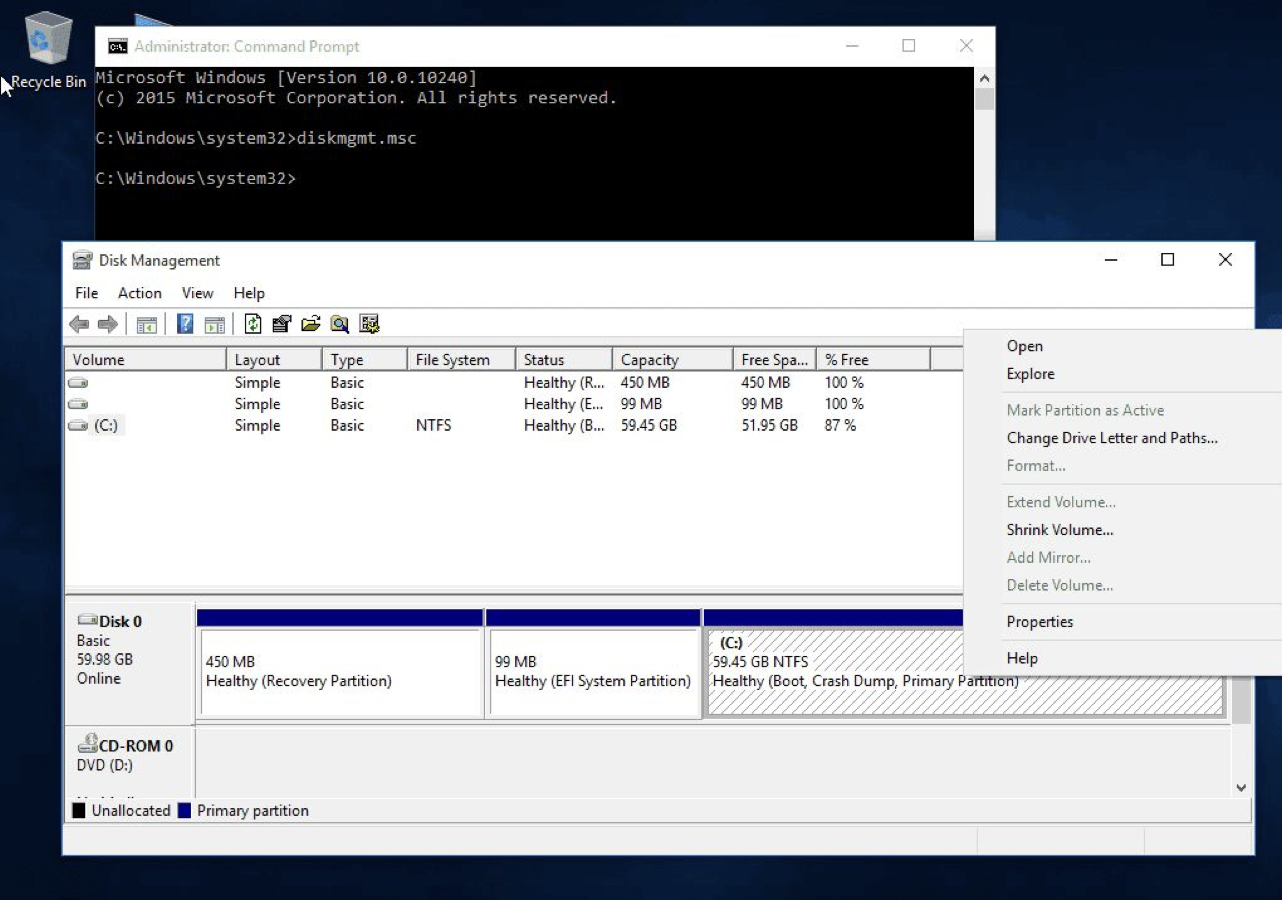
\includegraphics[width=0.6\linewidth]{images/step1.png}
        % \caption{Enter Caption}
        \label{fig:enter-label}
    \end{figure}
    \item Create space for Ubuntu:
    \begin{itemize}
        \item Right-click C: drive
        \item Select ``Shrink Volume''
        \item Enter minimum 60000 MB (60GB)
        \item Confirm shrink operation
    \end{itemize}
    \begin{figure}[htp]
        \centering
        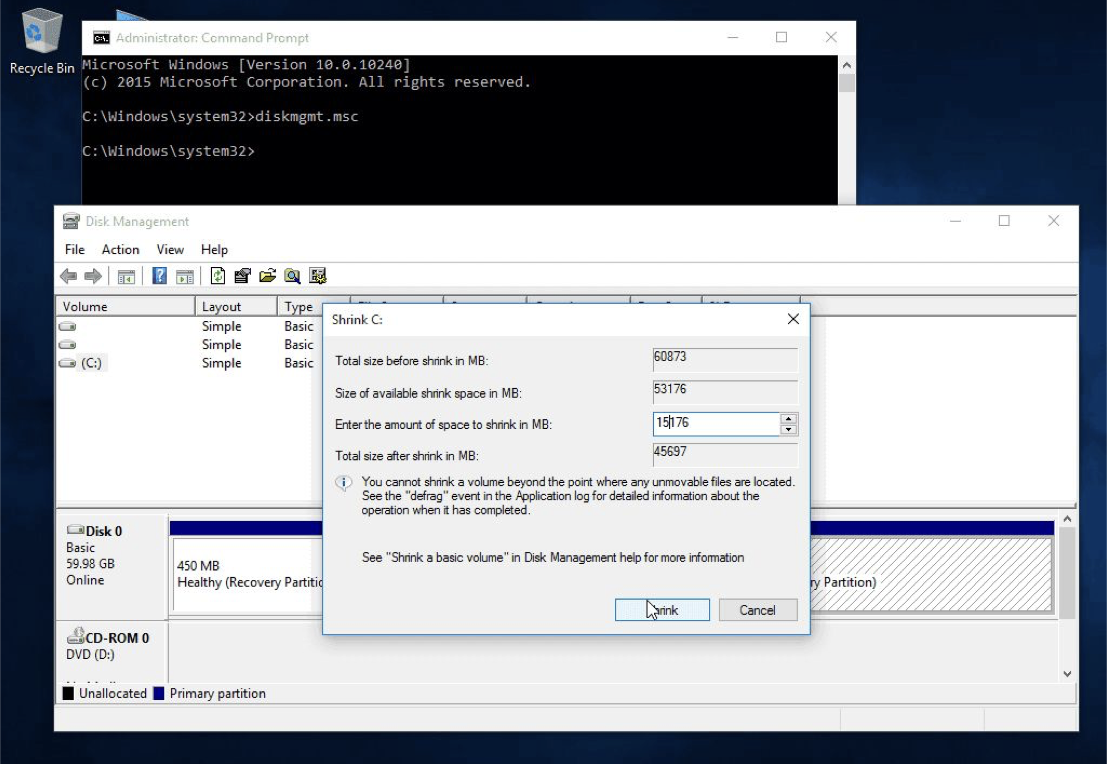
\includegraphics[width=0.6\linewidth]{images/step2.png}
        % \caption{Enter Caption}
        \label{fig:enter-label}
    \end{figure}
    Note: I have just added some random numbers in the above image but ensure that you allocate a minimum of 60GB free space.
    \item Leave the unallocated space as it is.
    \begin{figure}[htp]
        \centering
        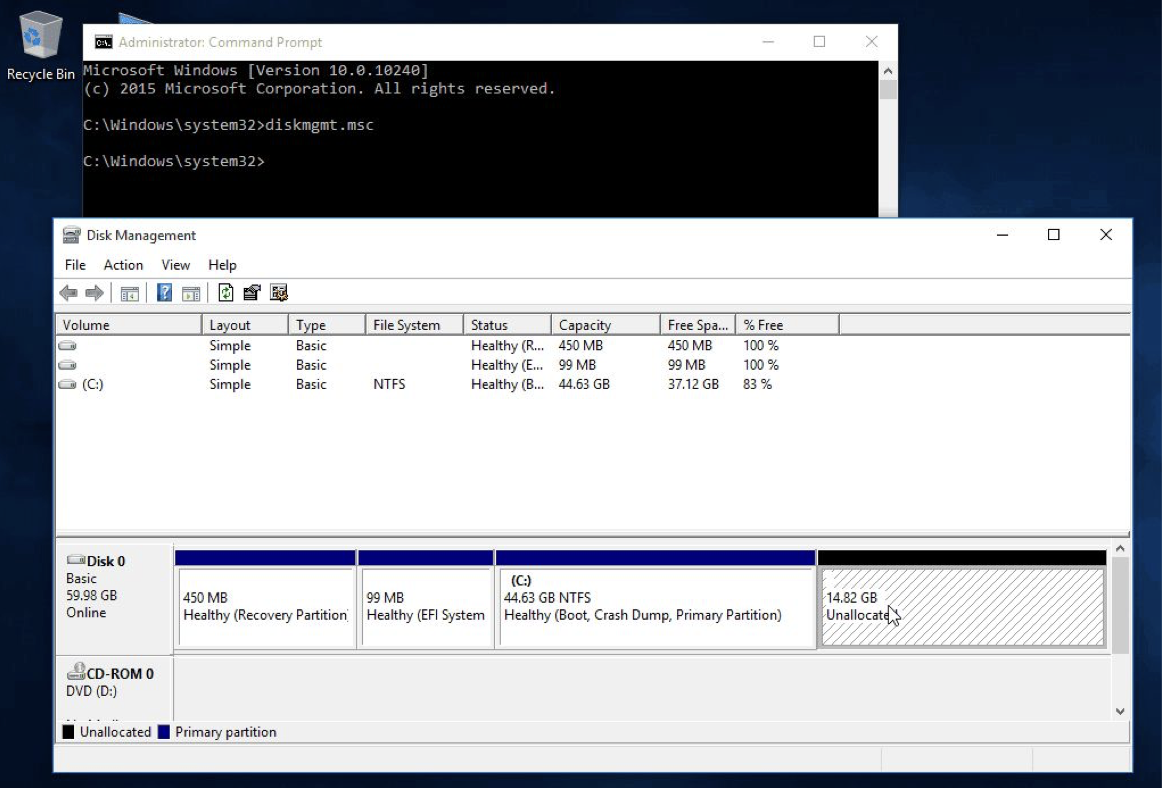
\includegraphics[width=0.6\linewidth]{images/step3.png}
        % \caption{Enter Caption}
        \label{fig:enter-label}
    \end{figure}
\end{enumerate}

\section{Ubuntu Installation Process}
\subsection{Creating Bootable USB}
\begin{enumerate}
    \item Launch Rufus
    \item Insert USB drive
    \item Configure Rufus:
    \begin{itemize}
        \item Select USB drive
        \item Choose downloaded Ubuntu ISO
        \item Keep default settings
        \item Click START
    \end{itemize}
\end{enumerate}
 Follow \href{https://rufus.ie/en/}{this guide} if needed.

\subsection{Booting Ubuntu Installer}
\begin{enumerate}
    \item Insert bootable USB
    \item Restart computer
    \item Enter boot menu (F2, F12, F10 or manufacturer-specific key)
    \item Select USB drive
    \item Choose ``Install Ubuntu'' from boot menu
    \begin{figure}[htp]
        \centering
        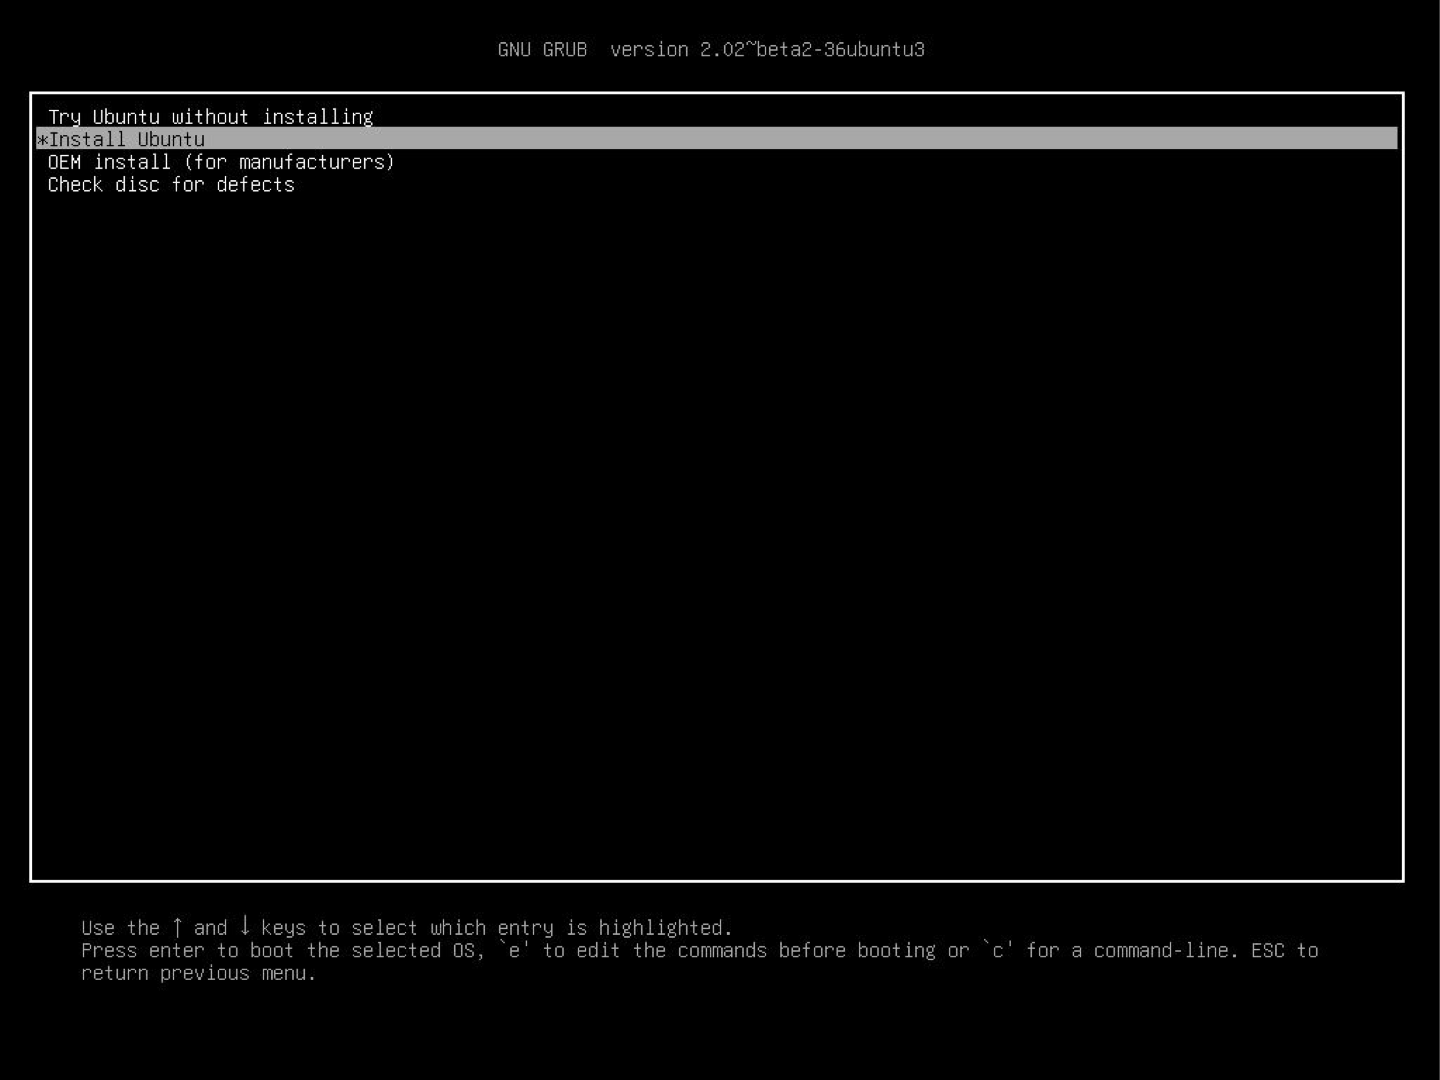
\includegraphics[width=0.6\linewidth]{images/step4.png}
        % \caption{Enter Caption}
        \label{fig:enter-label}
    \end{figure}
\end{enumerate}

\subsection{Installation Configuration}
Note: This is the most important part so do it carefully!
\begin{enumerate}
    \item Language Selection:
    \begin{itemize}
        \item Choose preferred language
        \item Click Continue
    \end{itemize}
    \begin{figure}[htp]
        \centering
        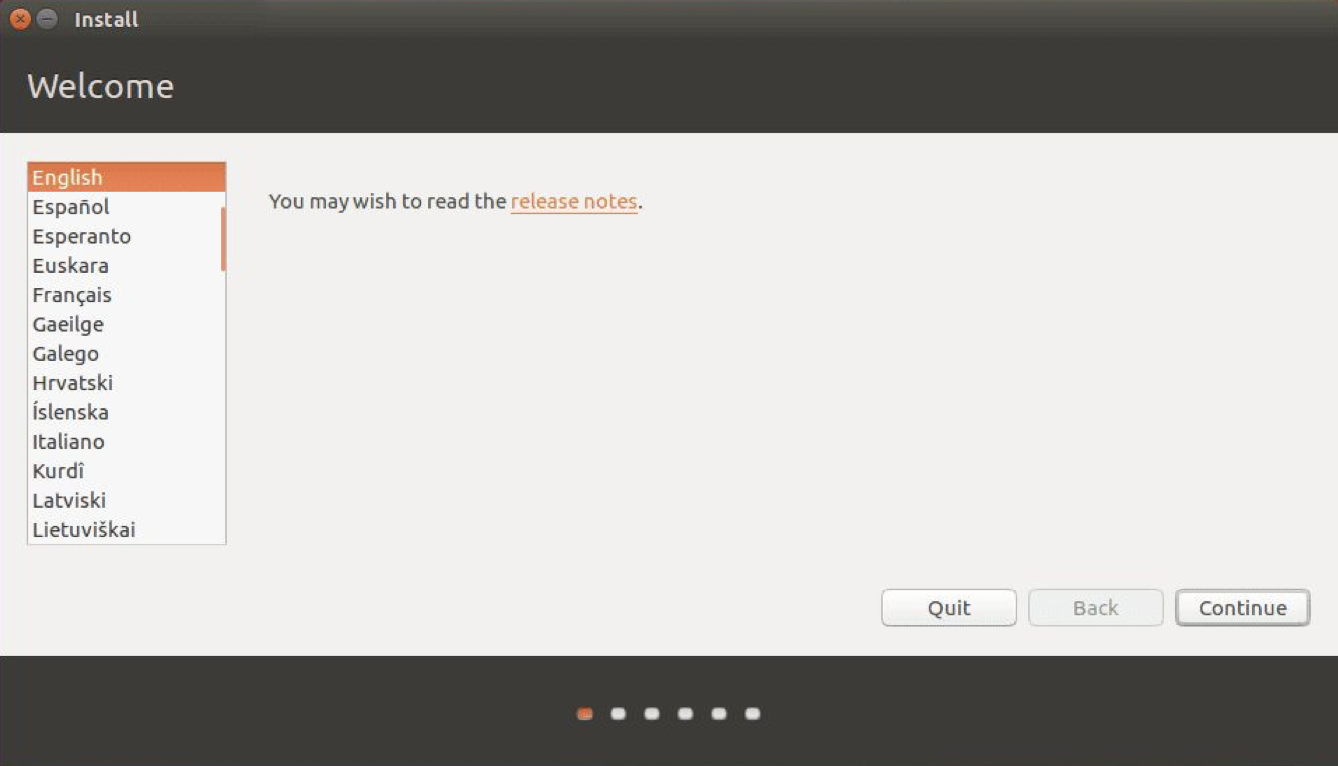
\includegraphics[width=0.4\linewidth]{images/step5.png}
        % \caption{Enter Caption}
        \label{fig:enter-label}
    \end{figure}
    
    \item Installation Type:
    \begin{itemize}
        \item Select ``Normal Installation''
        \item Enable ``Download updates while installing'' [Optional but Recommended]
        \item Enable ``Install third-party software'' [Optional but Recommended]
    \end{itemize}
    \begin{figure}[htp]
        \centering
        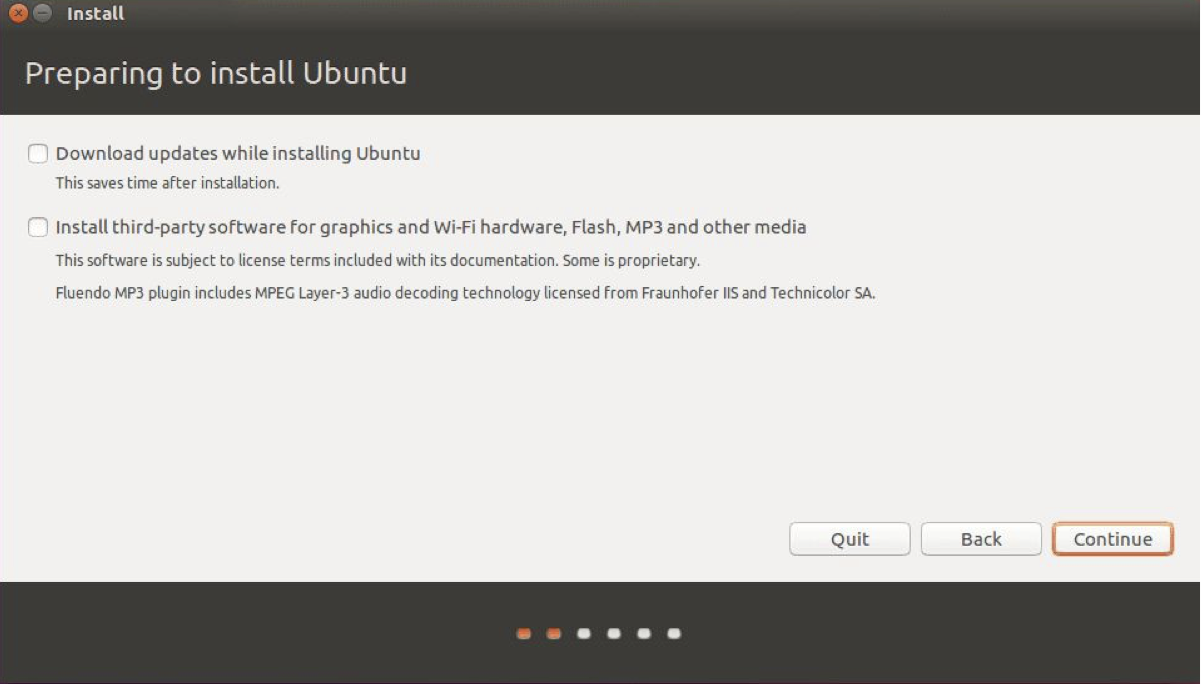
\includegraphics[width=0.6\linewidth]{images/step6.png}
        % \caption{Enter Caption}
        \label{fig:enter-label}
    \end{figure}
    I haven't selected these options but you should select both of these. 
    \begin{warning}
    Select ``Something Else'' for manual partitioning. Never select ``Erase disk and install Ubuntu''!
    \end{warning}
    \begin{figure}[htp]
        \centering
        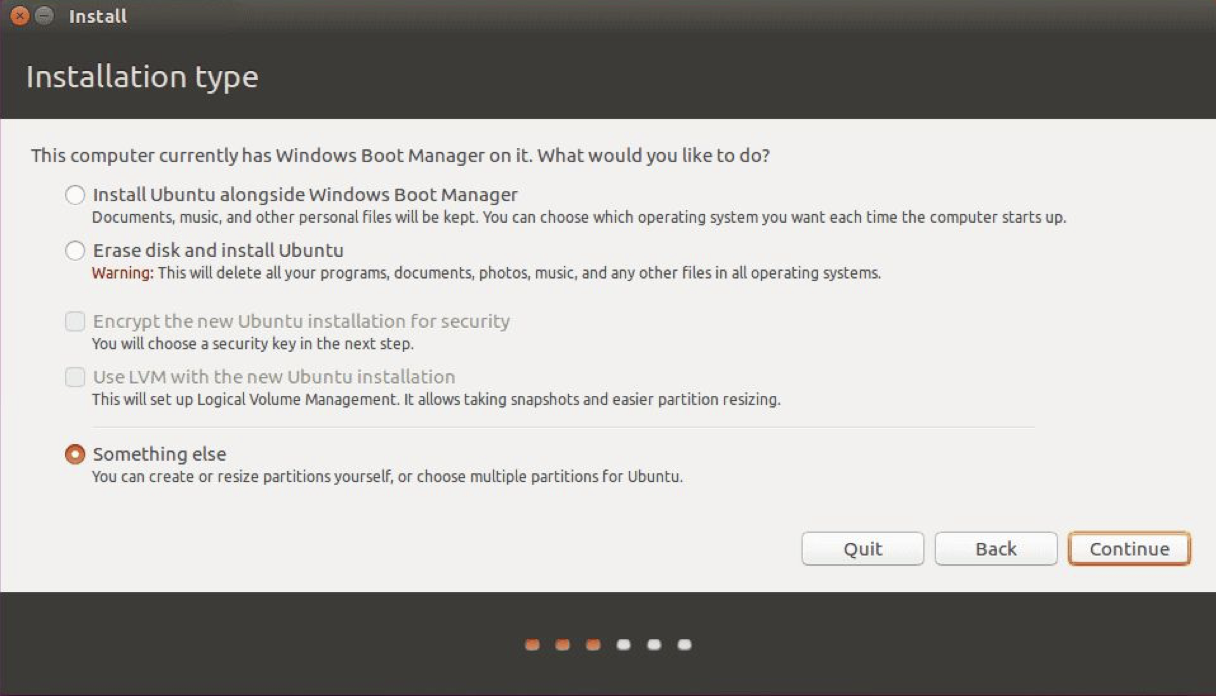
\includegraphics[width=0.6\linewidth]{images/step7.png}
        % \caption{Enter Caption}
        \label{fig:enter-label}
    \end{figure}
    \item Partition Setup:
    \begin{figure}[htp]
        \centering
        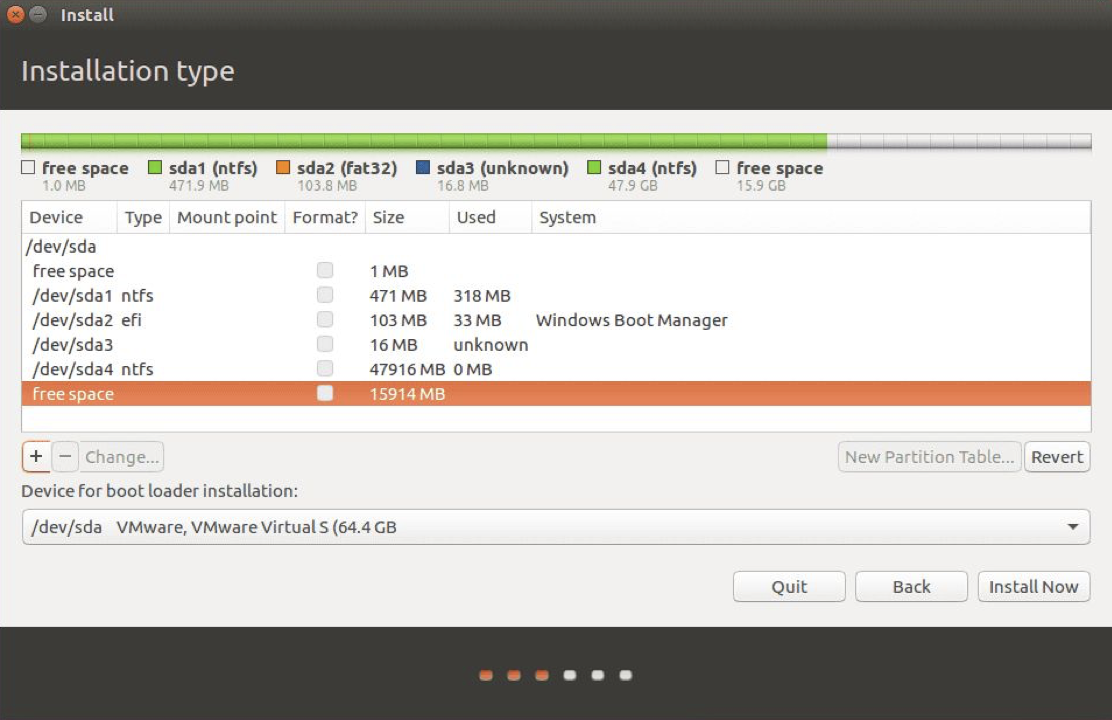
\includegraphics[width=0.6\linewidth]{images/step8.png}
        % \caption{Enter Caption}
        \label{fig:enter-label}
    \end{figure}
    \begin{itemize}
        \item Create Root Partition:
        To create the first partition, the root partition, select
the free space (the shrink space from Windows created
earlier) and hit on the + icon below. On partition settings
use the following configurations and hit OK to apply
changes:
        \begin{itemize}
            \item Size: Total free space minus 10000MB
            \item Type: Primary
            \item File System: EXT4
            \item Mount Point: /
        \end{itemize}
        
        \item Create Swap Partition:
        \begin{itemize}
            \item Size: 10000MB
            \item Type: Swap Area
        \end{itemize}
    \end{itemize}
    
    \begin{figure}[htp]
        \centering
        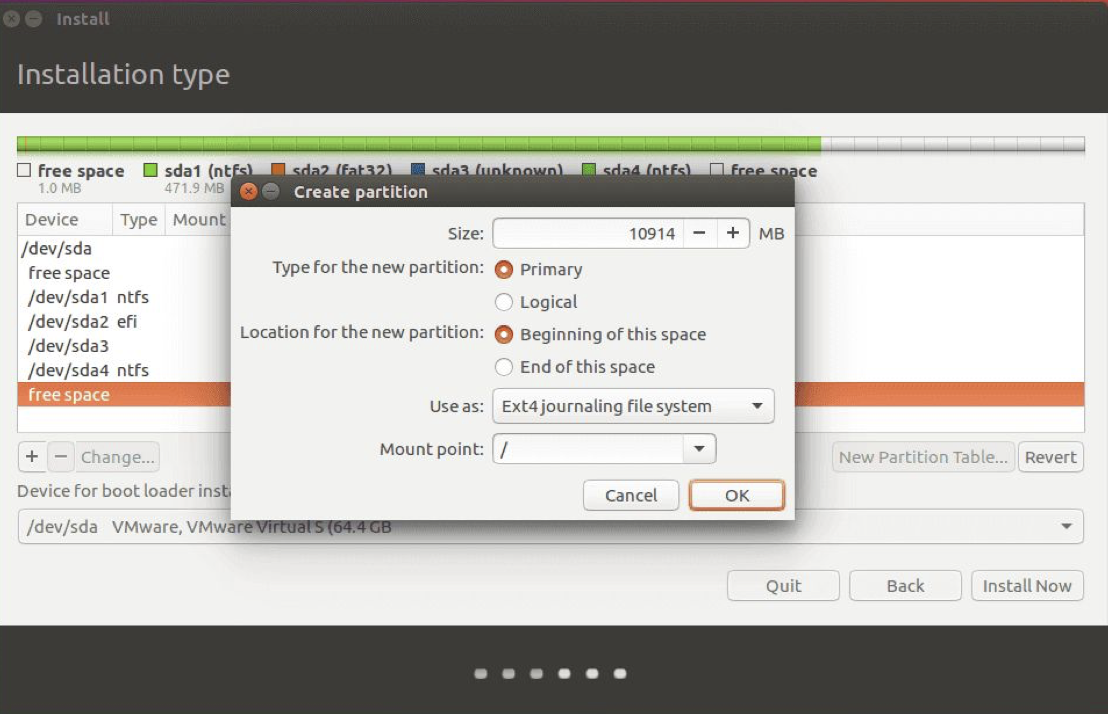
\includegraphics[width=0.6\linewidth]{images/step9.png}
        % \caption{Enter Caption}
        \label{fig:enter-label}
    \end{figure}
    \item When finished, hit the ``Install Now'' button in order to apply
changes to disk and start the installation process.
    \item A pop-up window should appear to inform you about swap
space. Ignore the alert by pressing on the ``Continue'' button.
Next, a new pop-up window will ask you if you agree with
committing changes to disk. Hit ``Continue'' to write changes
to disk and the installation process will now start.
\end{enumerate}

\section{Final steps}
\begin{itemize}
    \item On the next screen adjust your machine physical location
    by selecting a city nearby from the map. When done hit
    ``Continue'' to move ahead.
    \item Next, select your keyboard layout and click on the
``Continue'' button.
    \item Pick up a username and password for your administrative
sudo account, enter a descriptive name for your computer
and hit ``Continue'' to finalize the installation.
\begin{note}
    Remember this sudo (admin) password as you will be using it a lot for all the updates and installation requirements.
    \end{note}
\end{itemize}
From here on the installation process will run automatically until it reaches the end.
\section{Post-Installation Configuration}
\subsection{First Boot}
After installation completes:
\begin{enumerate}
    \item Restart system
    \item Remove USB drive when prompted
    \item GRUB bootloader will appear
    \begin{itemize}
        \item Select Ubuntu or Windows Boot Manager
    \end{itemize}
\end{enumerate}
\begin{figure}[htp]
        \centering
        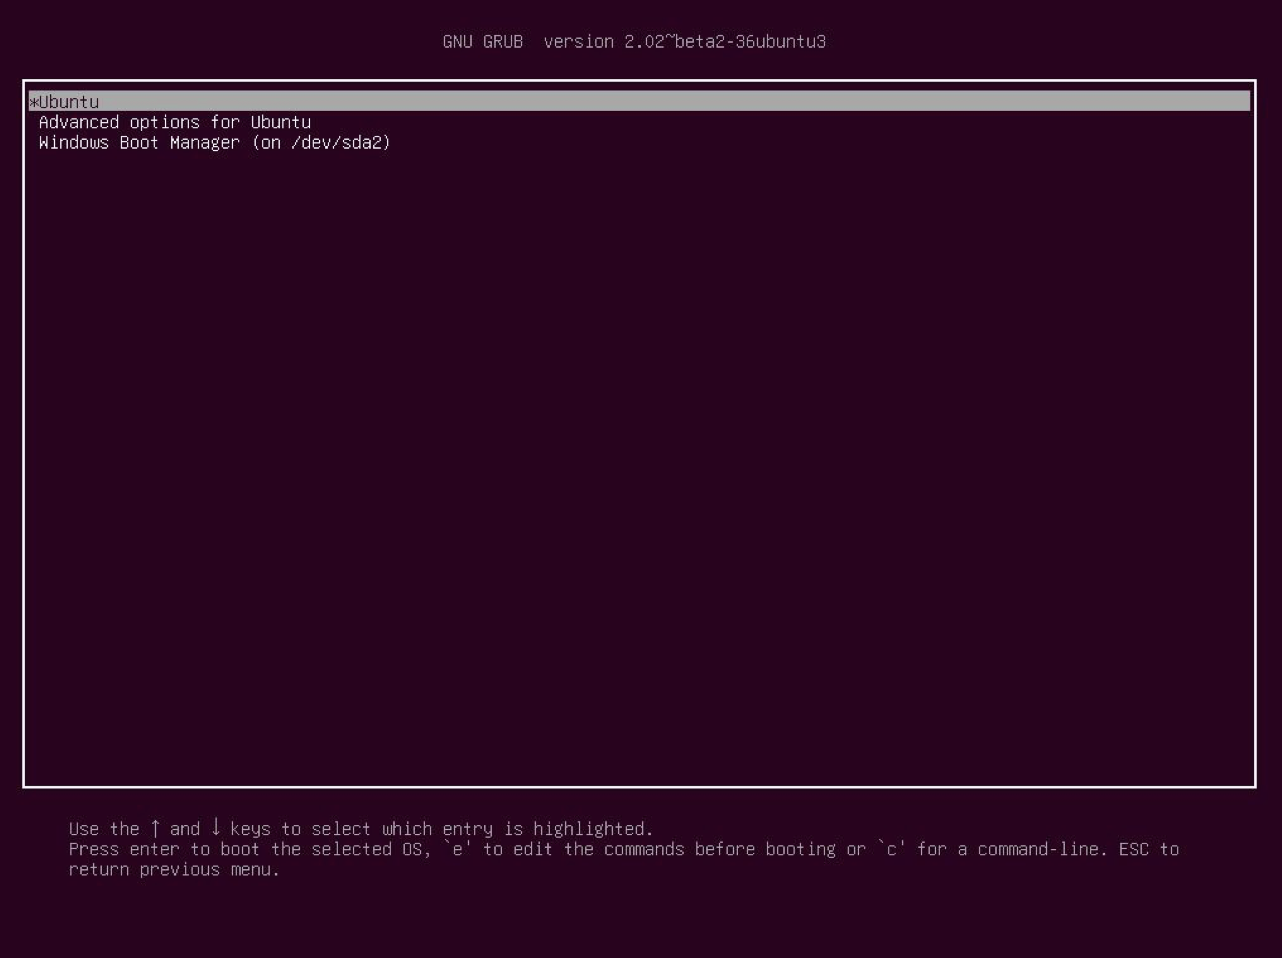
\includegraphics[width=0.6\linewidth]{images/step10.png}
        % \caption{Enter Caption}
        \label{fig:enter-label}
    \end{figure}

\subsection{Ubuntu Updates}
Open terminal and run:
\begin{lstlisting}
sudo apt-get update && sudo apt-get upgrade
sudo reboot
\end{lstlisting}

\section{Troubleshooting}
First contact TAs if there is any issue!
\subsection{Common Issues}
\begin{enumerate}
    \item GRUB Menu Not Appearing:
    \begin{itemize}
        \item Hold SHIFT during boot
        \item If persistent, repair GRUB using live USB
    \end{itemize}
    
    \item Windows Not Booting:
    \begin{itemize}
        \item Check if Secure Boot is properly disabled
        \item Verify Windows partition wasn't modified
    \end{itemize}
    
    \item Ubuntu Not Booting:
    \begin{itemize}
        \item Check partition mounting points
        \item Verify GRUB installation location
    \end{itemize}
\end{enumerate}

\section{Best Practices}
\subsection{Regular Maintenance}
\begin{itemize}
    \item Keep both systems updated
    \item Maintain adequate free space on both partitions
    \item Create regular backups
    \item Test both systems after major updates
\end{itemize}

\subsection{File Sharing}
\begin{itemize}
    \item Windows partitions are accessible from Ubuntu
    \item Create a shared data partition (optional)
    \item Use cloud storage for cross-platform file access
\end{itemize}

\section{Remarks}
Following this guide should result in a properly configured dual-boot system. Remember to:
\begin{itemize}
    \item Always backup important data
    \item Follow instructions carefully
    \item Keep both systems updated
    \item Document any custom configurations
\end{itemize}

It will reboot your system and you are good to go now! Welcome to the Linux family!

\noindent\rule{\textwidth}{1pt}

\newpage
\part{Parallels Installation for Mac}

\section{Prerequisites for Mac Installation}
\subsection{System Requirements}
Before beginning the Parallels installation, ensure your Mac meets these requirements:
\begin{itemize}
    \item Intel or M-series Mac processor
    \item Minimum 20GB free disk space
    \item Active internet connection
    \item Administrative access to your Mac
\end{itemize}

\subsection{Required Software and Accounts}
\begin{itemize}
    \item Parallels Desktop software (\href{https://www.parallels.com}{Parallels website})
    \item Parallels account
    \item Ubuntu ISO file (correct version for your processor):
    \begin{itemize}
        \item \textbf{Intel Macs:} Standard x86-64 version from \href{https://releases.ubuntu.com/noble/}{Ubuntu releases}
        \item \textbf{M-series Macs:} ARM64 version from \href{https://ubuntu.com/download/server/arm}{Ubuntu ARM releases}
    \end{itemize}
\end{itemize}

\section{Preparing for Installation}
\subsection{Downloading Required Files}
\begin{enumerate}
    \item Download Ubuntu ISO:
    \begin{itemize}
        \item Intel Macs: Standard x86-64 version
        \item M-series Macs: ARM64 version
    \end{itemize}
    \item Download Parallels Desktop from \href{https://www.parallels.com}{Parallels website}.
\end{enumerate}

\section{Parallels Desktop Installation}
\subsection{Installing Parallels}
\begin{enumerate}
    \item Mount the Parallels Desktop $.dmg$ file:
    \begin{itemize}
        \item Double-click the downloaded $.dmg$
        \item Drag Parallels Desktop to Applications folder
    \end{itemize}
    \item Initial Setup:
    \begin{itemize}
        \item Launch Parallels from Applications
        \item Follow the setup wizard
        \item Sign in with Parallels account
        \item Use free account for sign in and initial installation and ignore license key when prompted
    \end{itemize}
\end{enumerate}

\section{Creating Ubuntu Virtual Machine}
\subsection{Virtual Machine Setup}
\begin{enumerate}
    \item Launch New VM Wizard:
    \begin{itemize}
        \item Click \textbf{File $\rightarrow$ New}
        \item Select \textbf{Install Windows or another OS}
        \begin{figure}[htp]
            \centering
            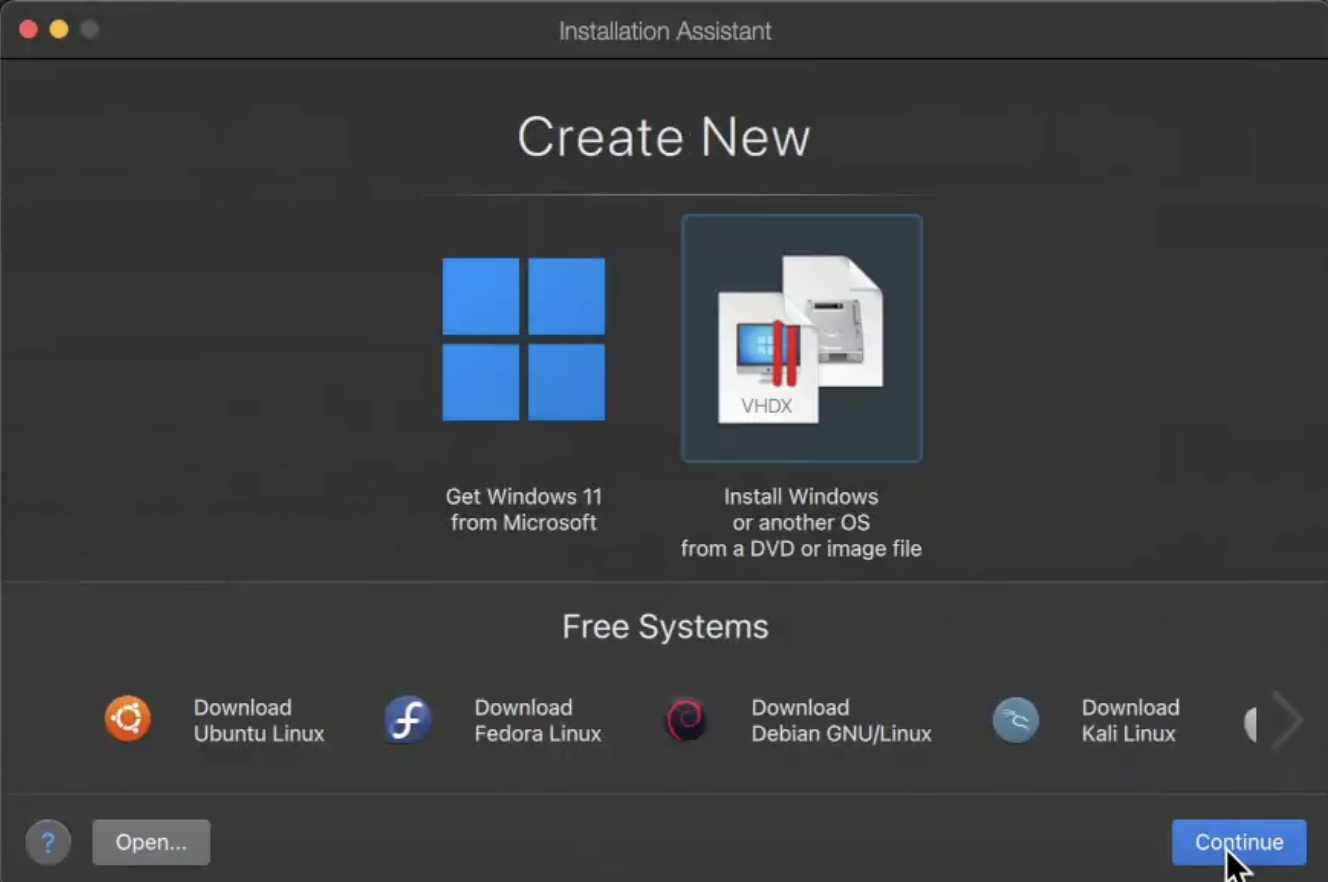
\includegraphics[width=0.6\linewidth]{images/step11.png}
        \end{figure}
    \end{itemize}
    \item Configure Installation Source:
    \begin{itemize}
        \item Choose \textbf{Install from DVD or image file}
        \item Select downloaded Ubuntu ISO
        \begin{figure}[htp]
            \centering
            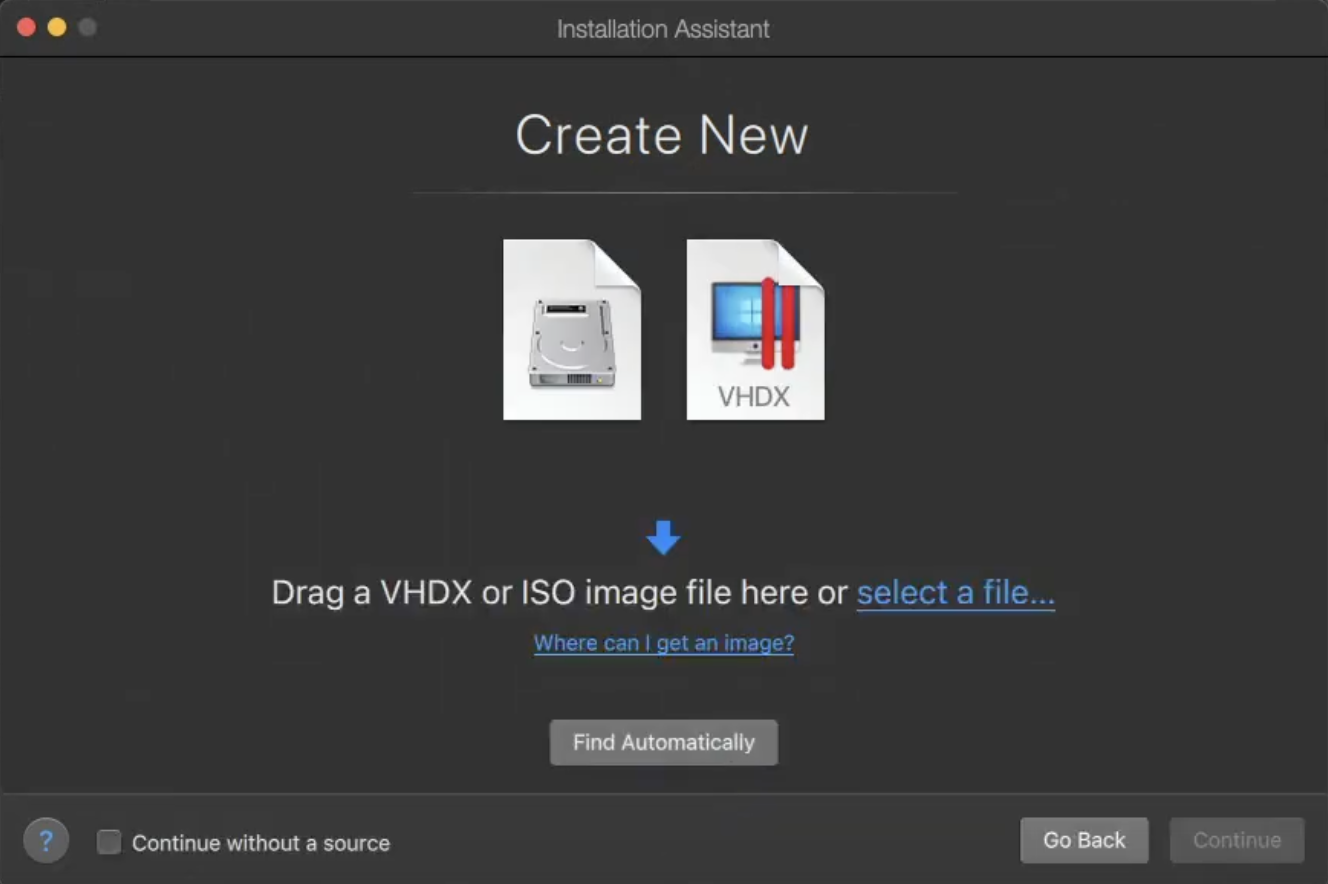
\includegraphics[width=0.6\linewidth]{images/step12.png}
        \end{figure}
    \end{itemize}
    \item Virtual Machine Configuration:
    \begin{itemize}
        \item Name: Choose descriptive name
        \item Location: Select storage location
        \item Resource allocation:
        \begin{itemize}
            \item CPU: Minimum 2 cores
            \item RAM: Minimum 4GB
            \item Storage: Minimum 20GB
        \end{itemize}
        \begin{figure}[htp]
            \centering
            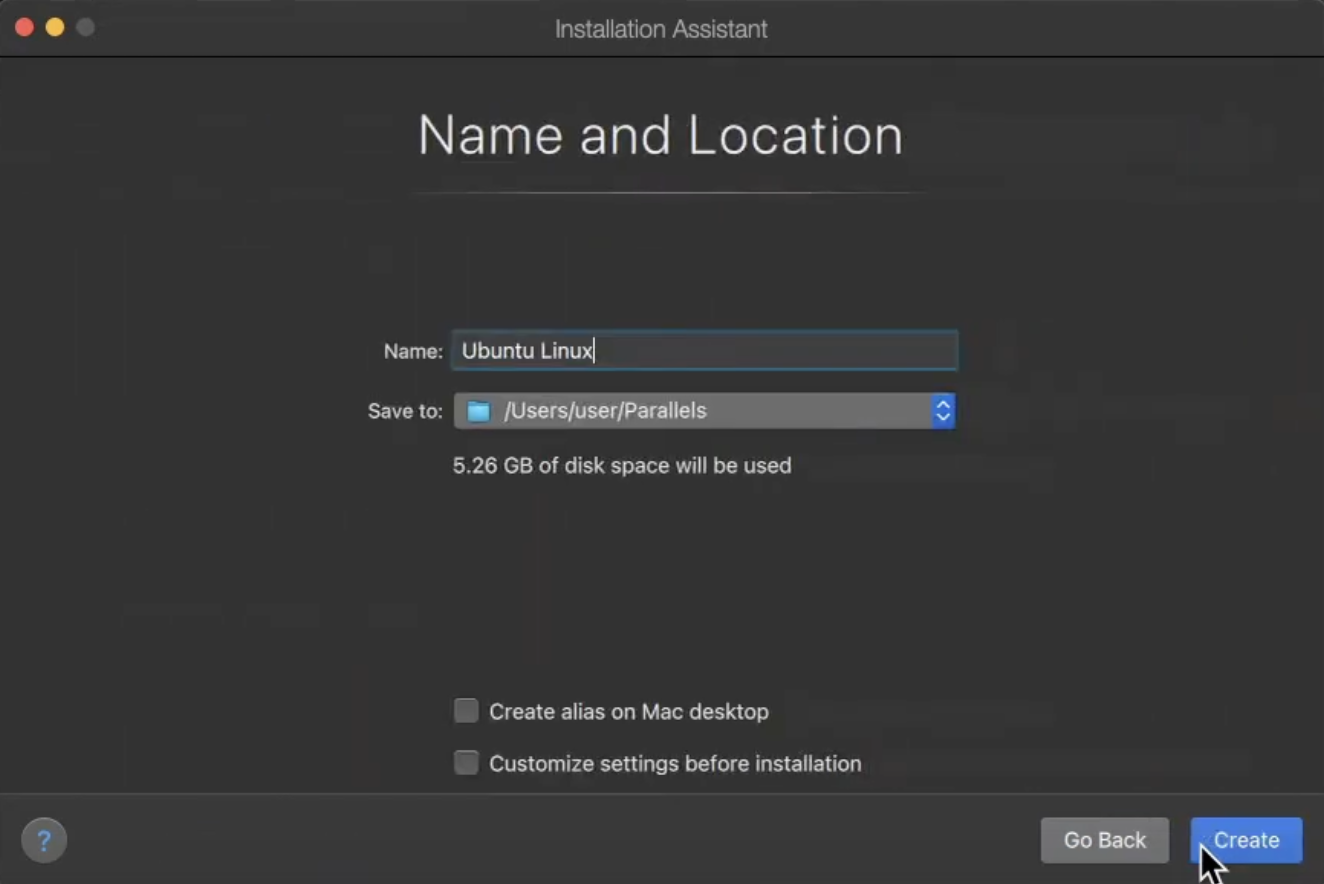
\includegraphics[width=0.6\linewidth]{images/step13.png}
        \end{figure}
    \end{itemize}
\end{enumerate}

\section{Ubuntu Installation in Parallels}
\subsection{Start the Virtual Machine}
    \begin{itemize}
        \item Select your newly created virtual machine and click ``Start.''
        \item Choose Try or Install Ubuntu Server
    \end{itemize}
        \begin{figure}[htp]
            \centering
            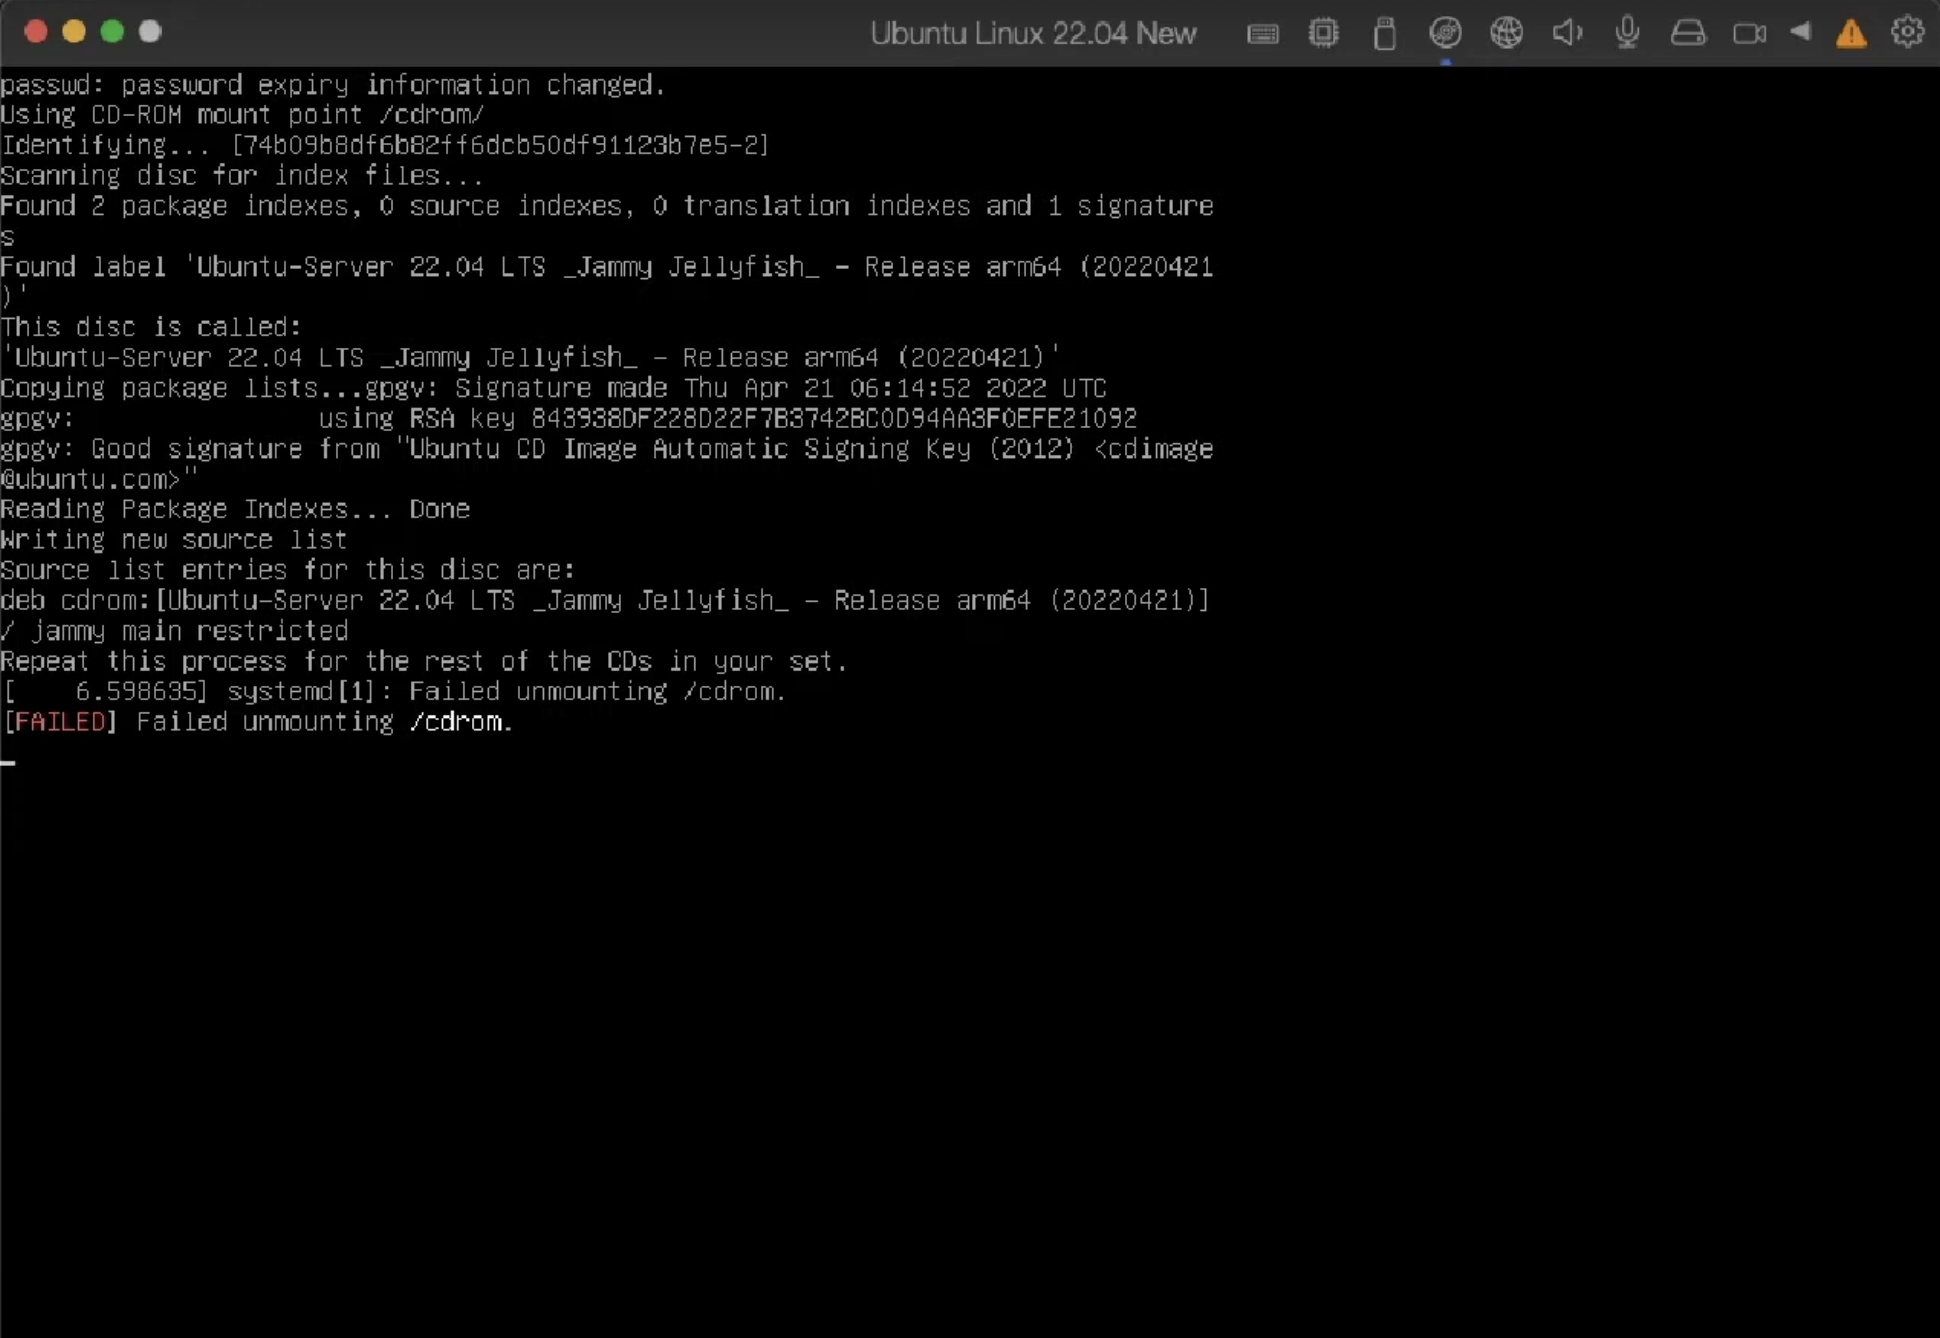
\includegraphics[width=0.6\linewidth]{images/step14.png}
        \end{figure}
\subsection{Installation Process}
\begin{enumerate}
    \item Initial Setup:
    \begin{itemize}
        \item Select your language
        \begin{figure}[htp]
            \centering
            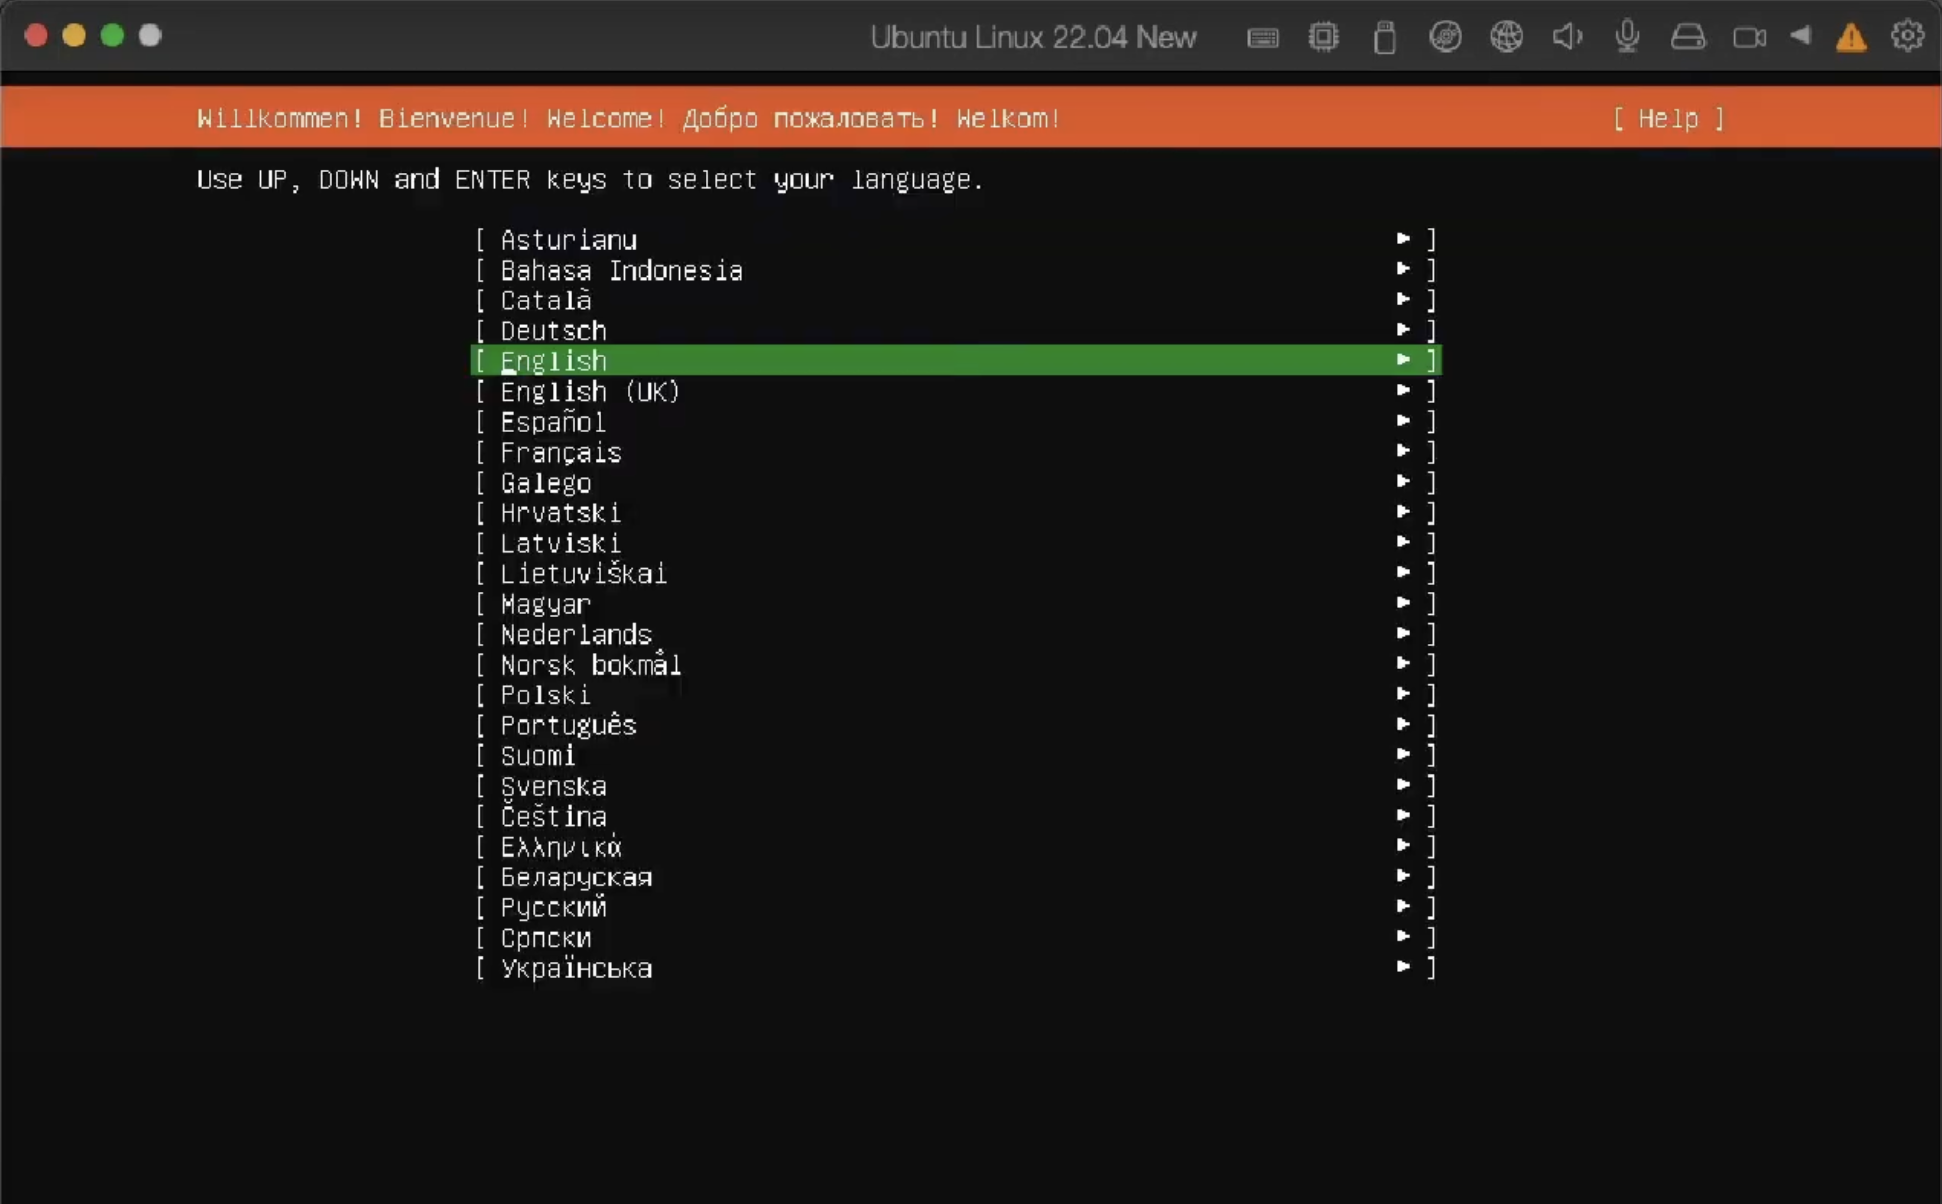
\includegraphics[width=0.35\linewidth]{images/step15.png}
        \end{figure}
        \item Check Download updates while installing Ubuntu and Install third-party software (optional but recommended).
        \item Keep pressing ``Done''(without entering anything) until you reach:
        \begin{figure}[htp]
            \centering
            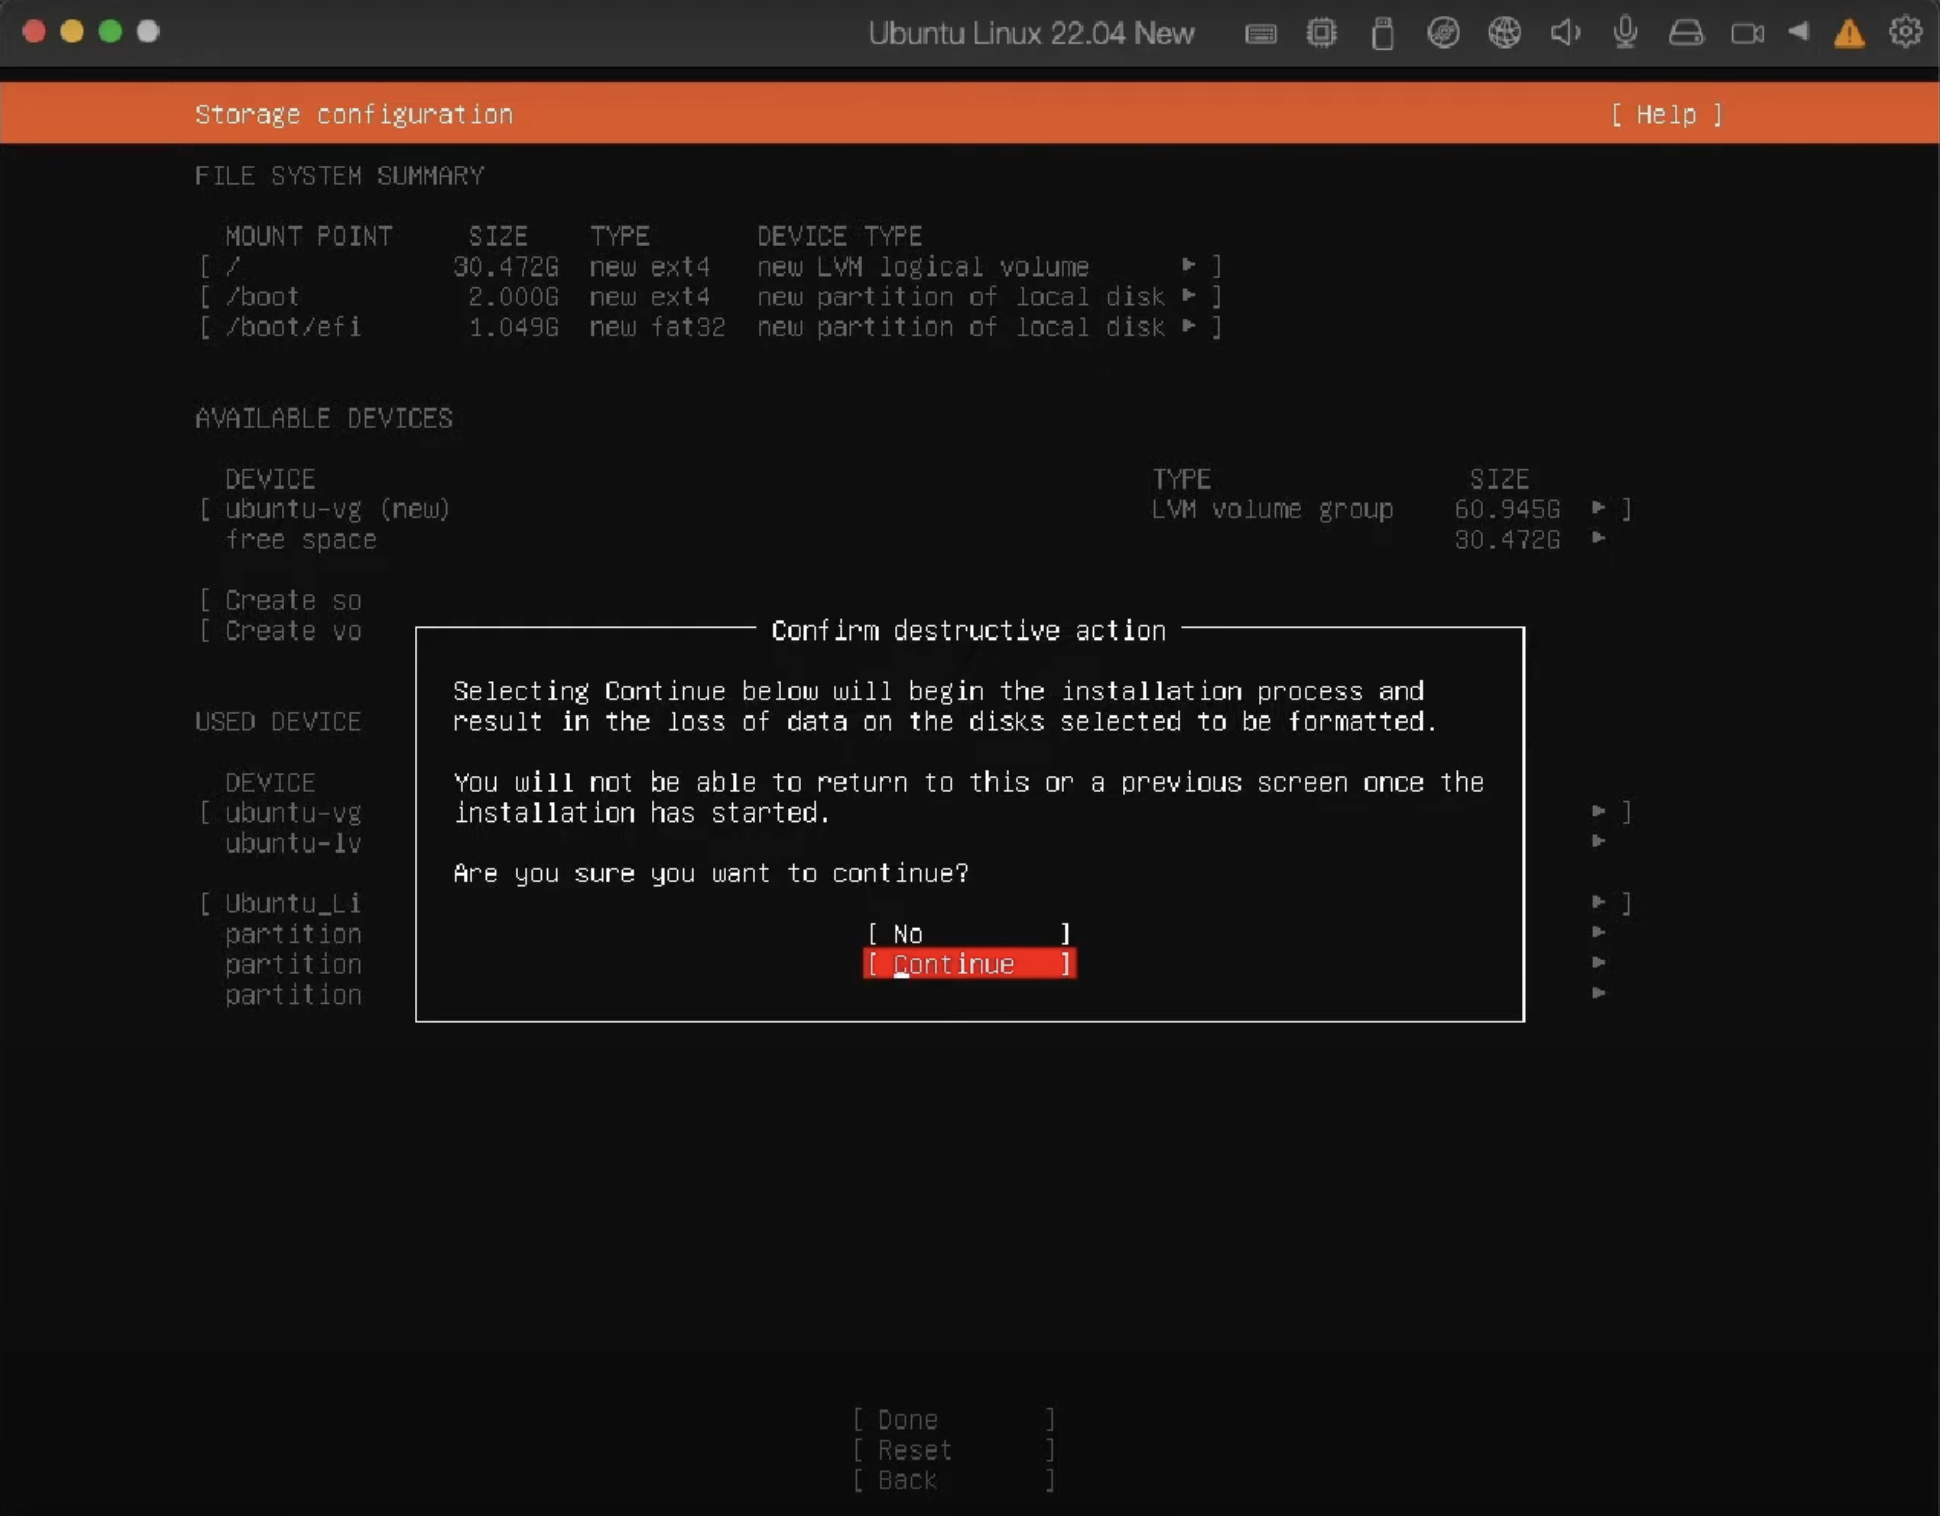
\includegraphics[width=0.6\linewidth]{images/step17.png}
        \end{figure}
        \item Press ``Continue''
    \end{itemize}
    
    \item User Setup:
    \begin{itemize}
        \item Create username and password
        \item Choose computer name
        \begin{figure}[htp]
            \centering
            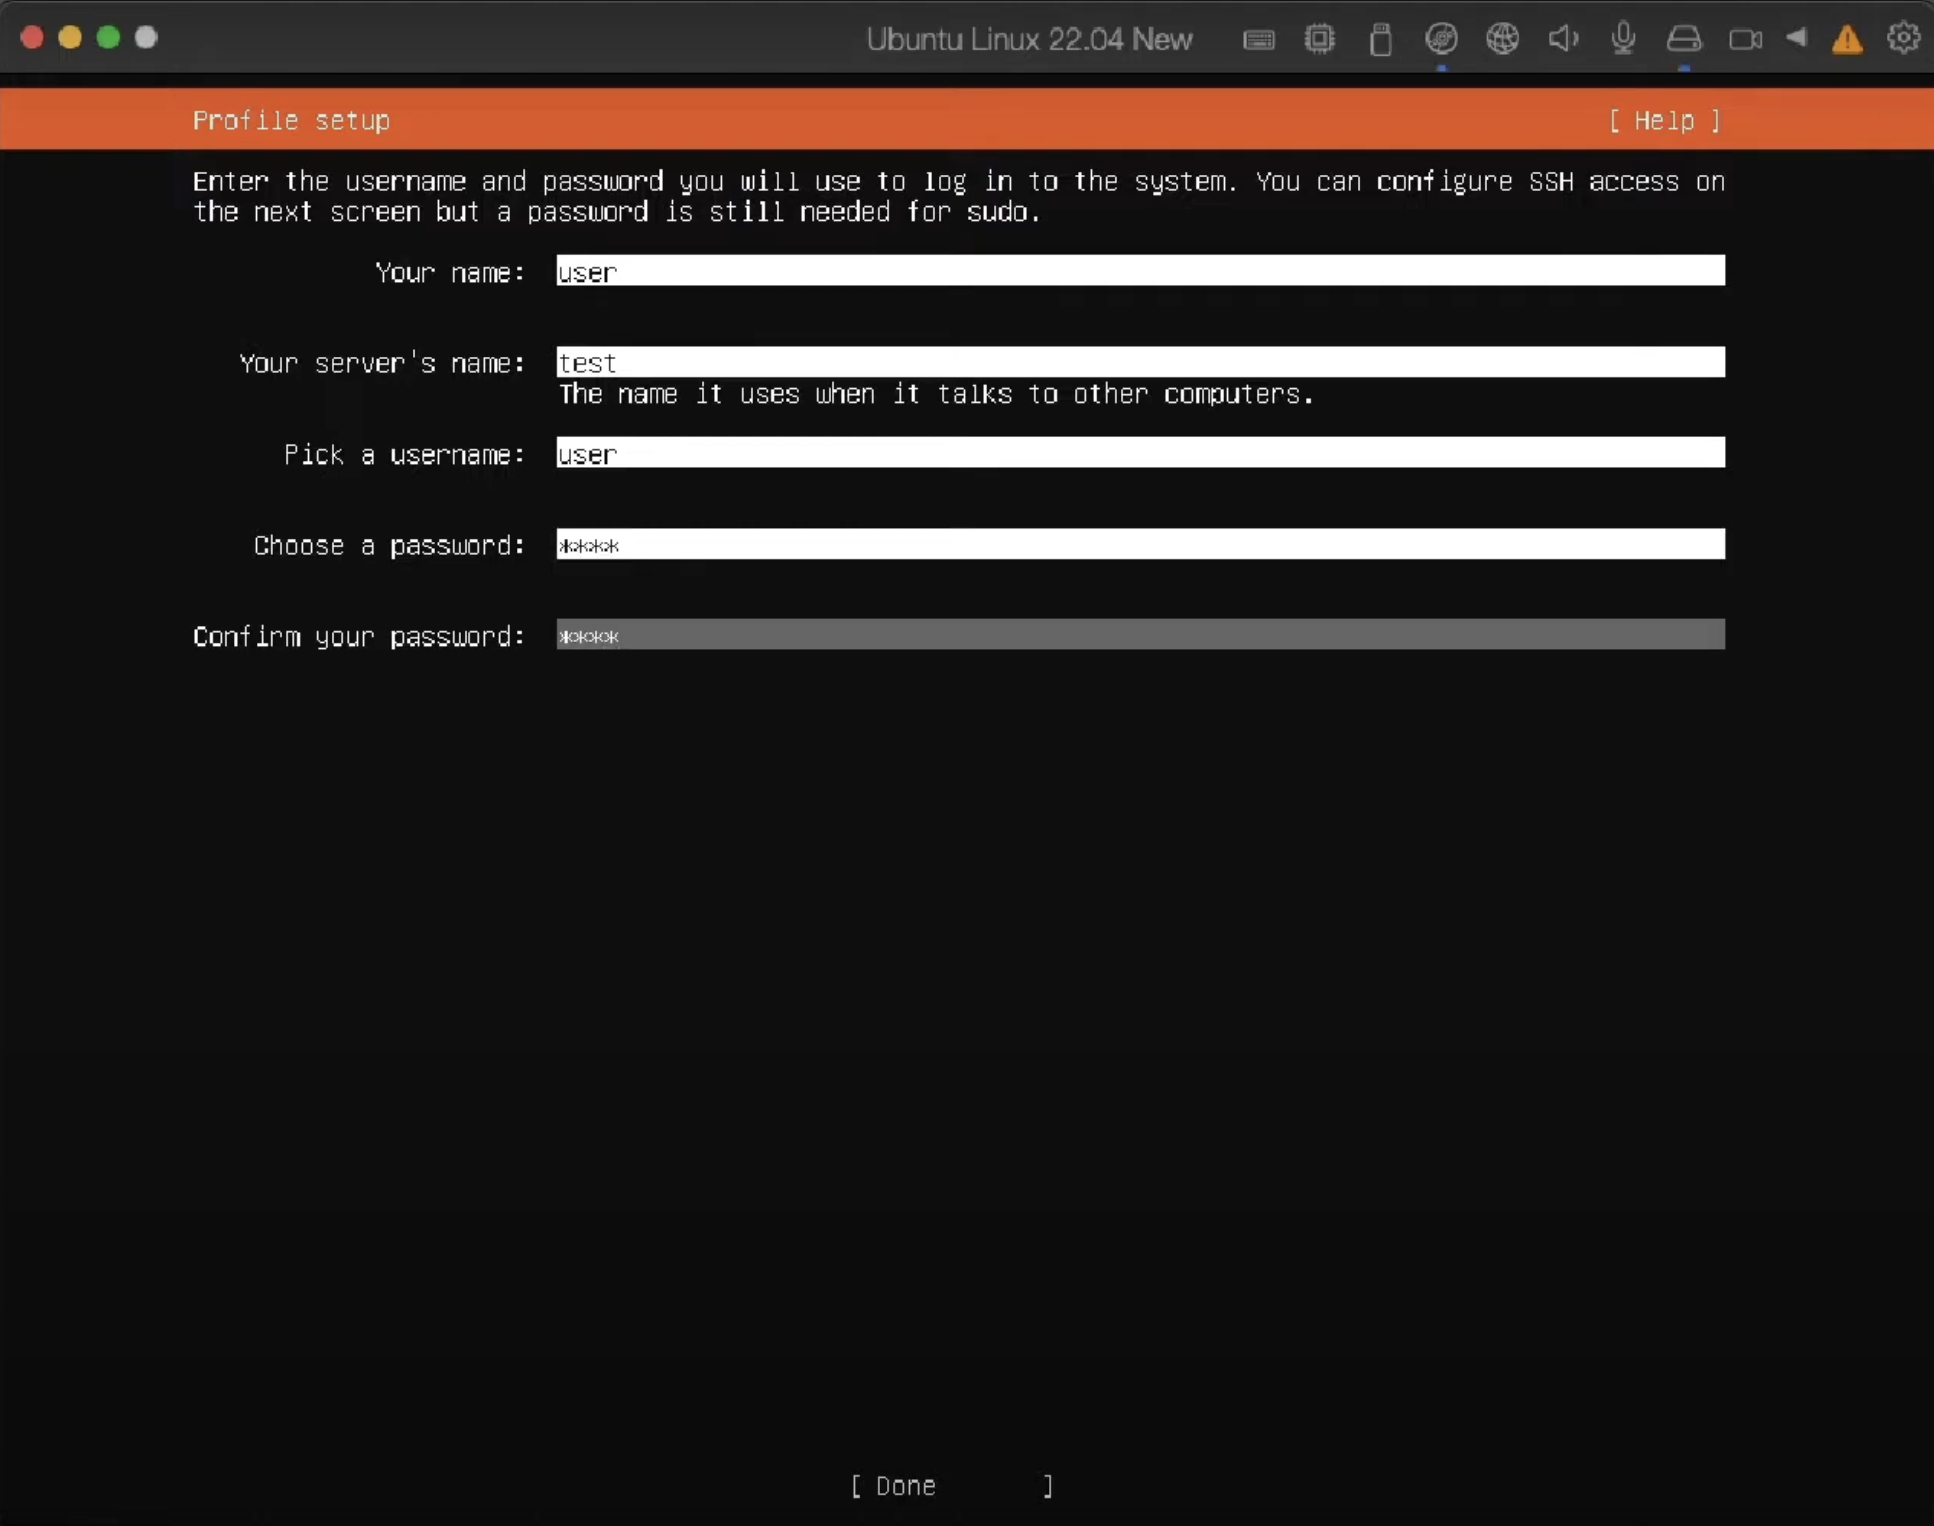
\includegraphics[width=0.6\linewidth]{images/step18.png}
        \end{figure}
    \end{itemize}
    \item Complete installation:
    \begin{itemize}
        \item Wait for the installation to complete
        \item Click Reboot Now when prompted
        \begin{figure}[htp]
            \centering
            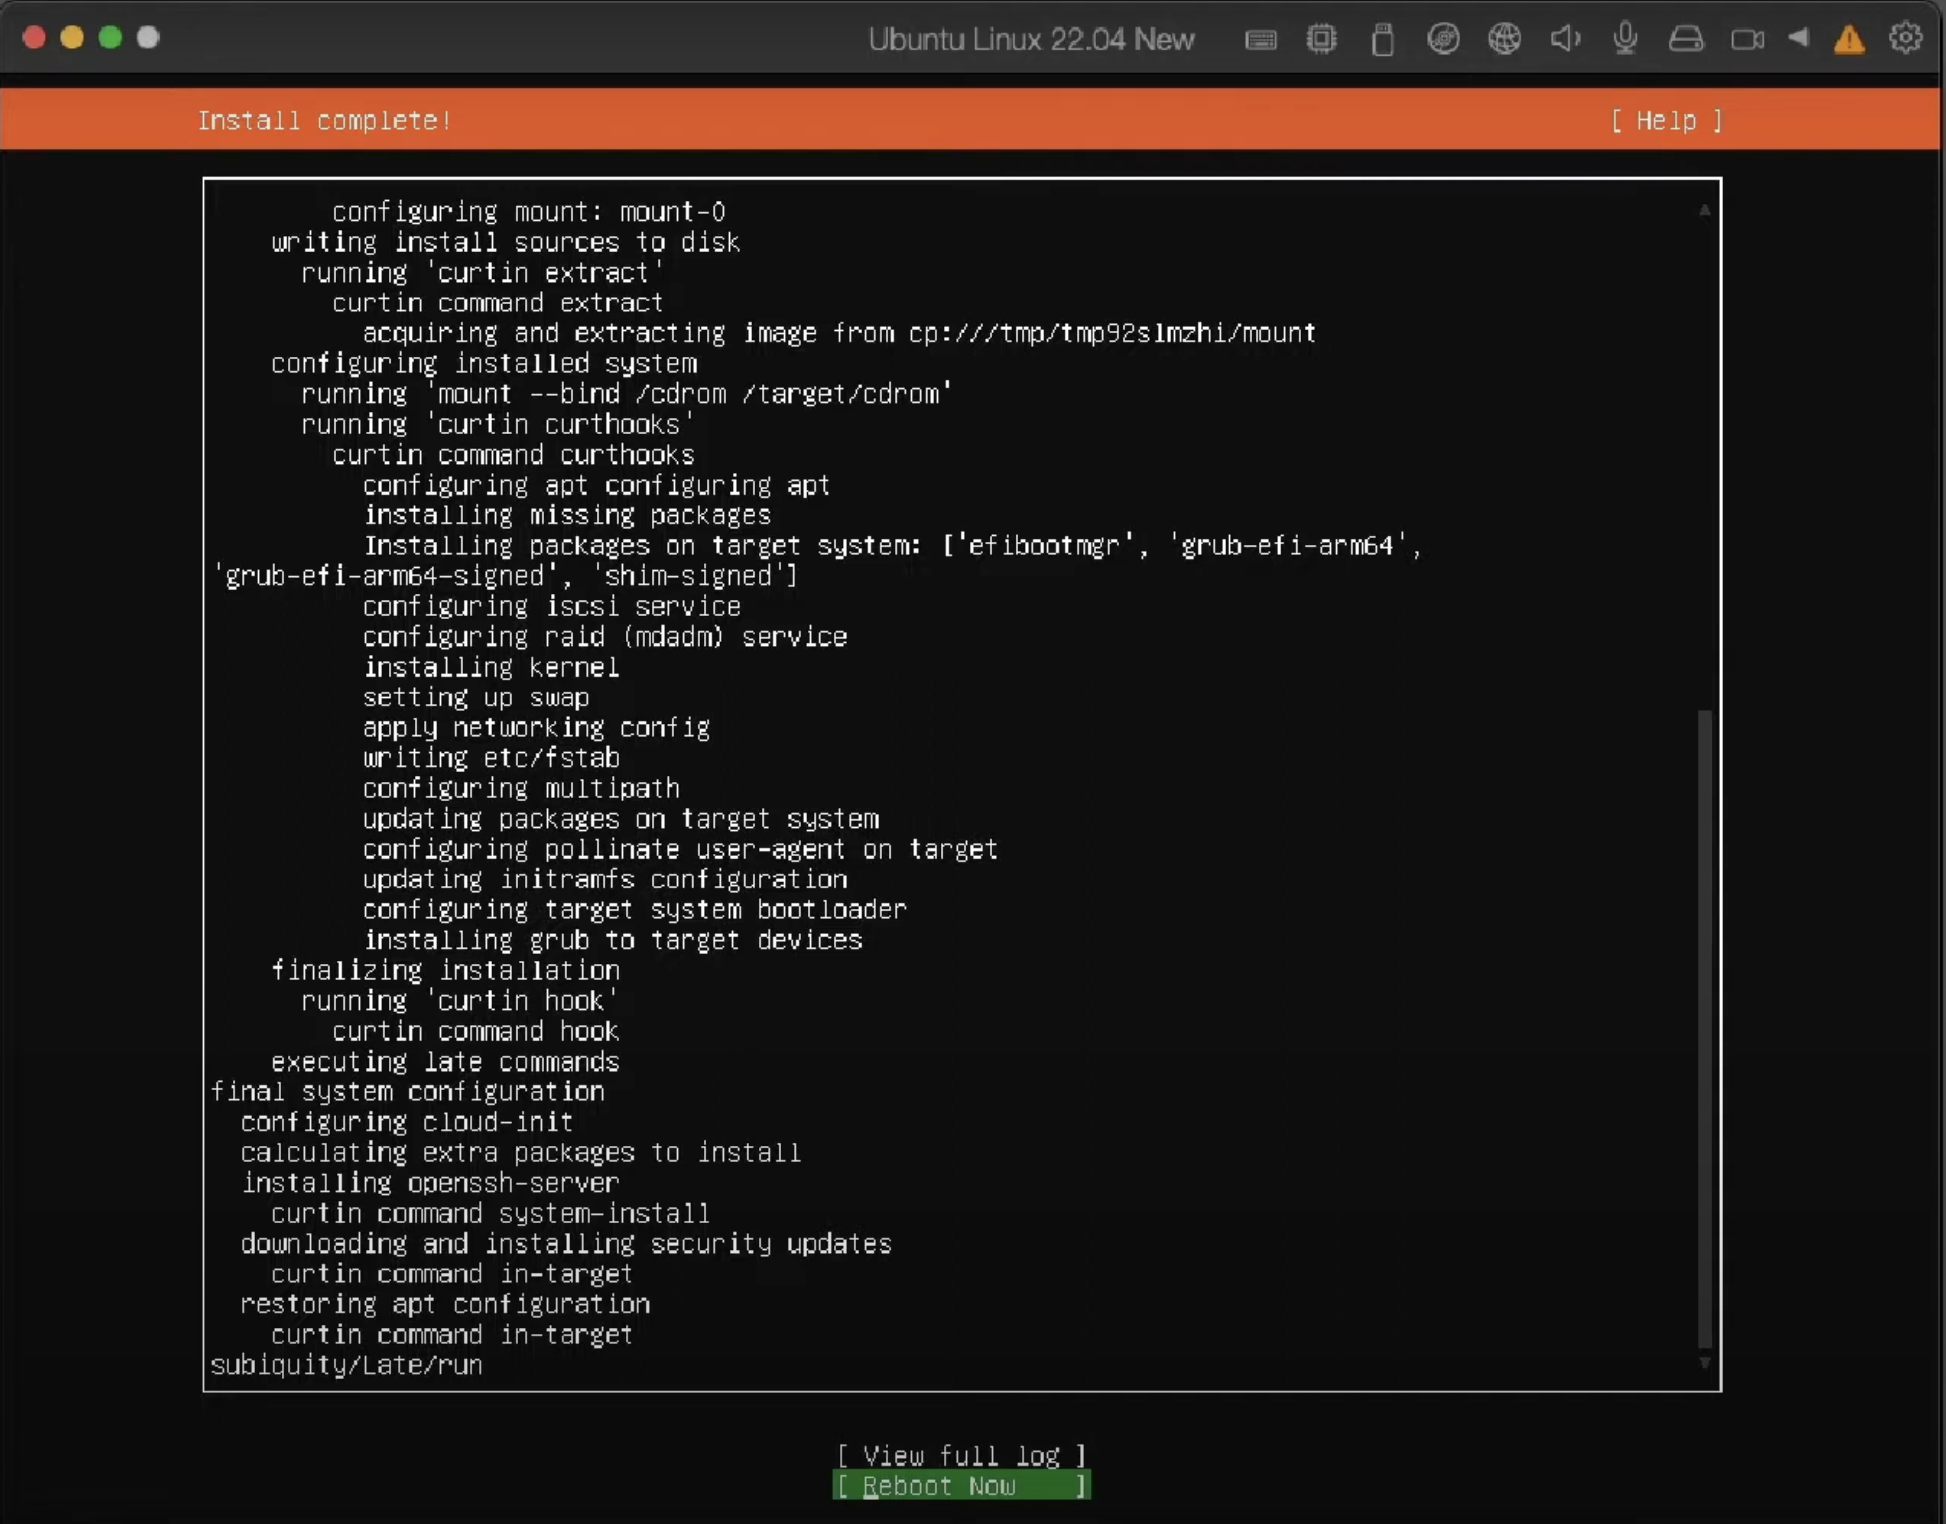
\includegraphics[width=0.5\linewidth]{images/step19.png}
        \end{figure}
    \end{itemize}
\end{enumerate}

% \section{Post-Installation Configuration}
% \subsection{Parallels Tools Installation}
% \begin{enumerate}
%     \item Install Parallels Tools:
%     \begin{lstlisting}
%     Actions -> Install Parallels Tools
%     \end{lstlisting}
%     \item Follow installation wizard
%     \item Restart virtual machine when prompted
% \end{enumerate}

\subsection{System Updates}
\begin{enumerate}
    \item You will be prompted for user and login password which you chose above.
    \begin{figure}[htp]
            \centering
            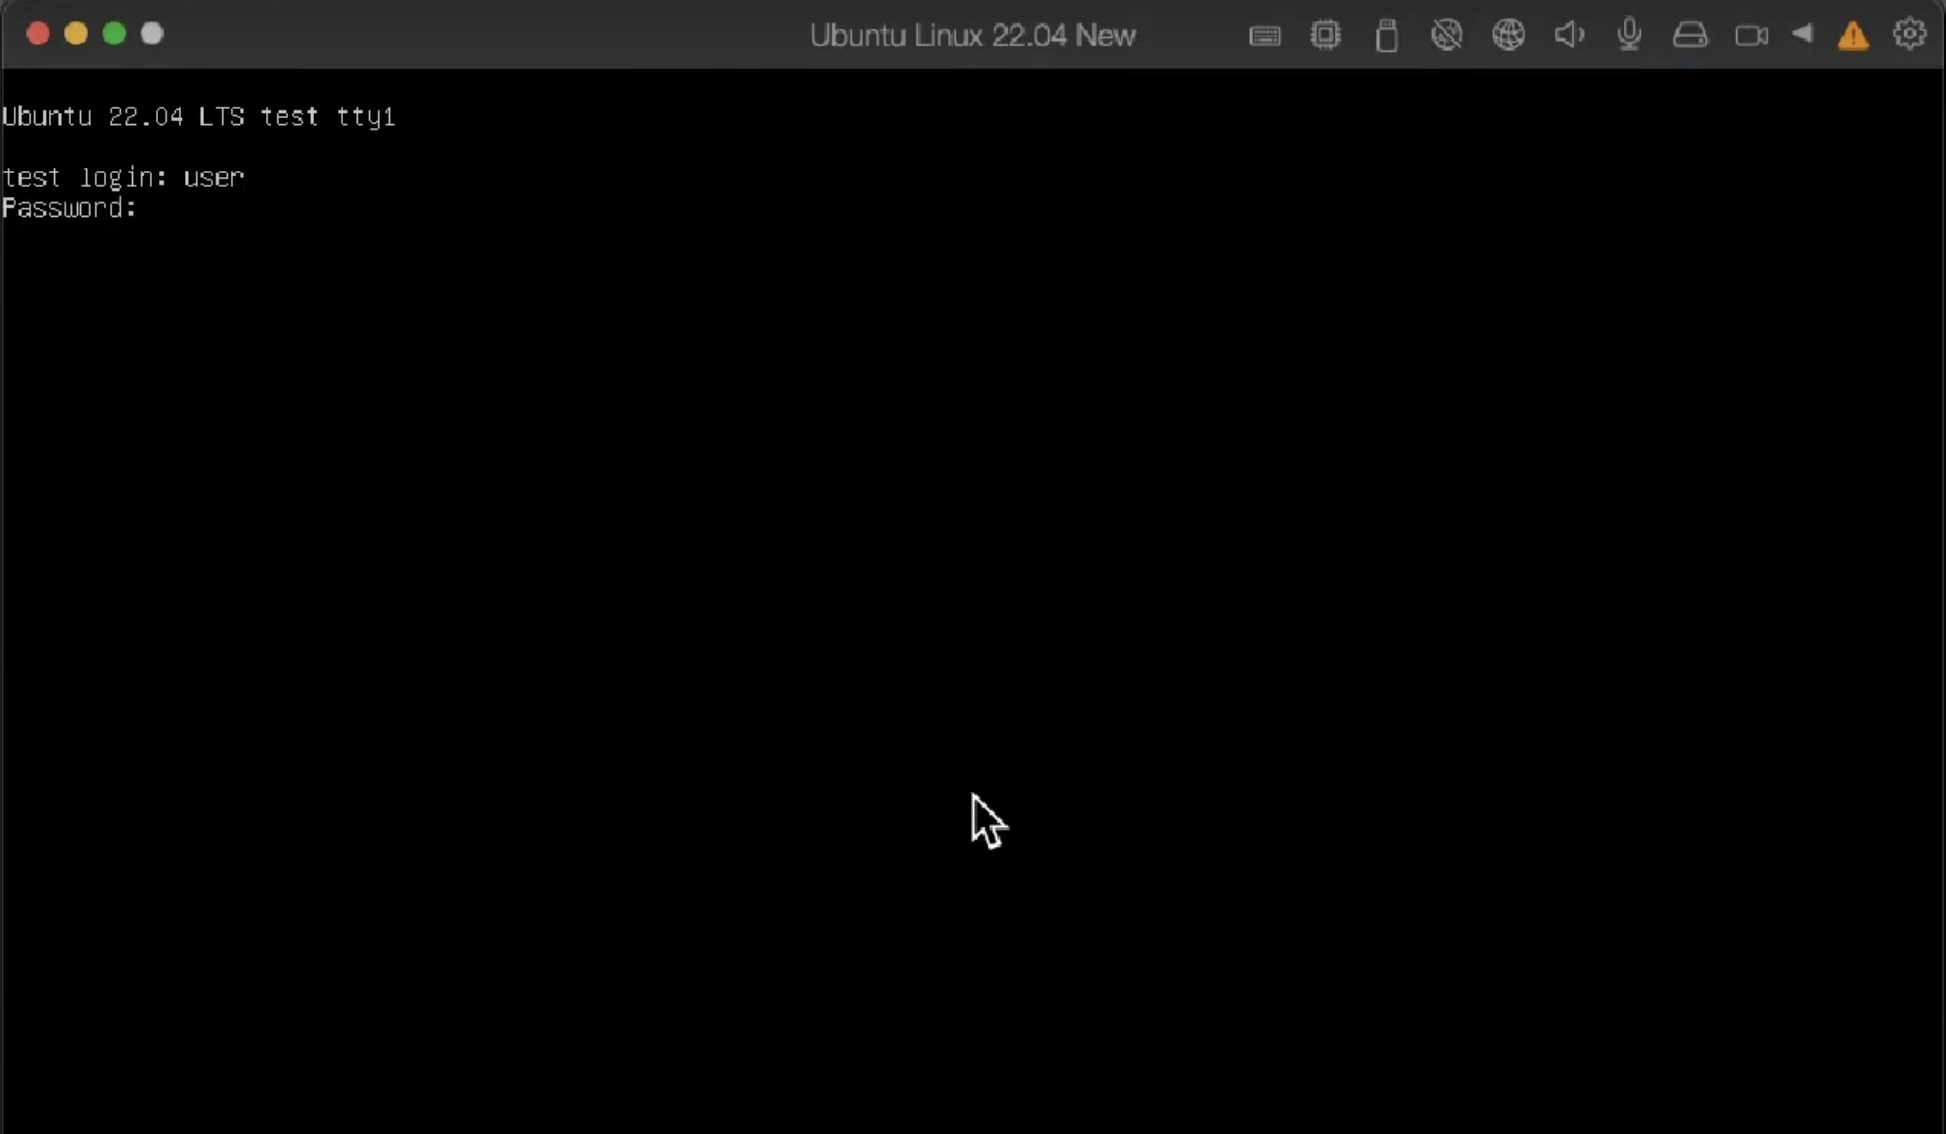
\includegraphics[width=0.5\linewidth]{images/step20.png}
        \end{figure}

    \item Open a terminal (Ctrl+Alt+T) and run:
\begin{lstlisting}
sudo apt update && sudo apt upgrade
\end{lstlisting}
    \begin{figure}[htp]
            \centering
            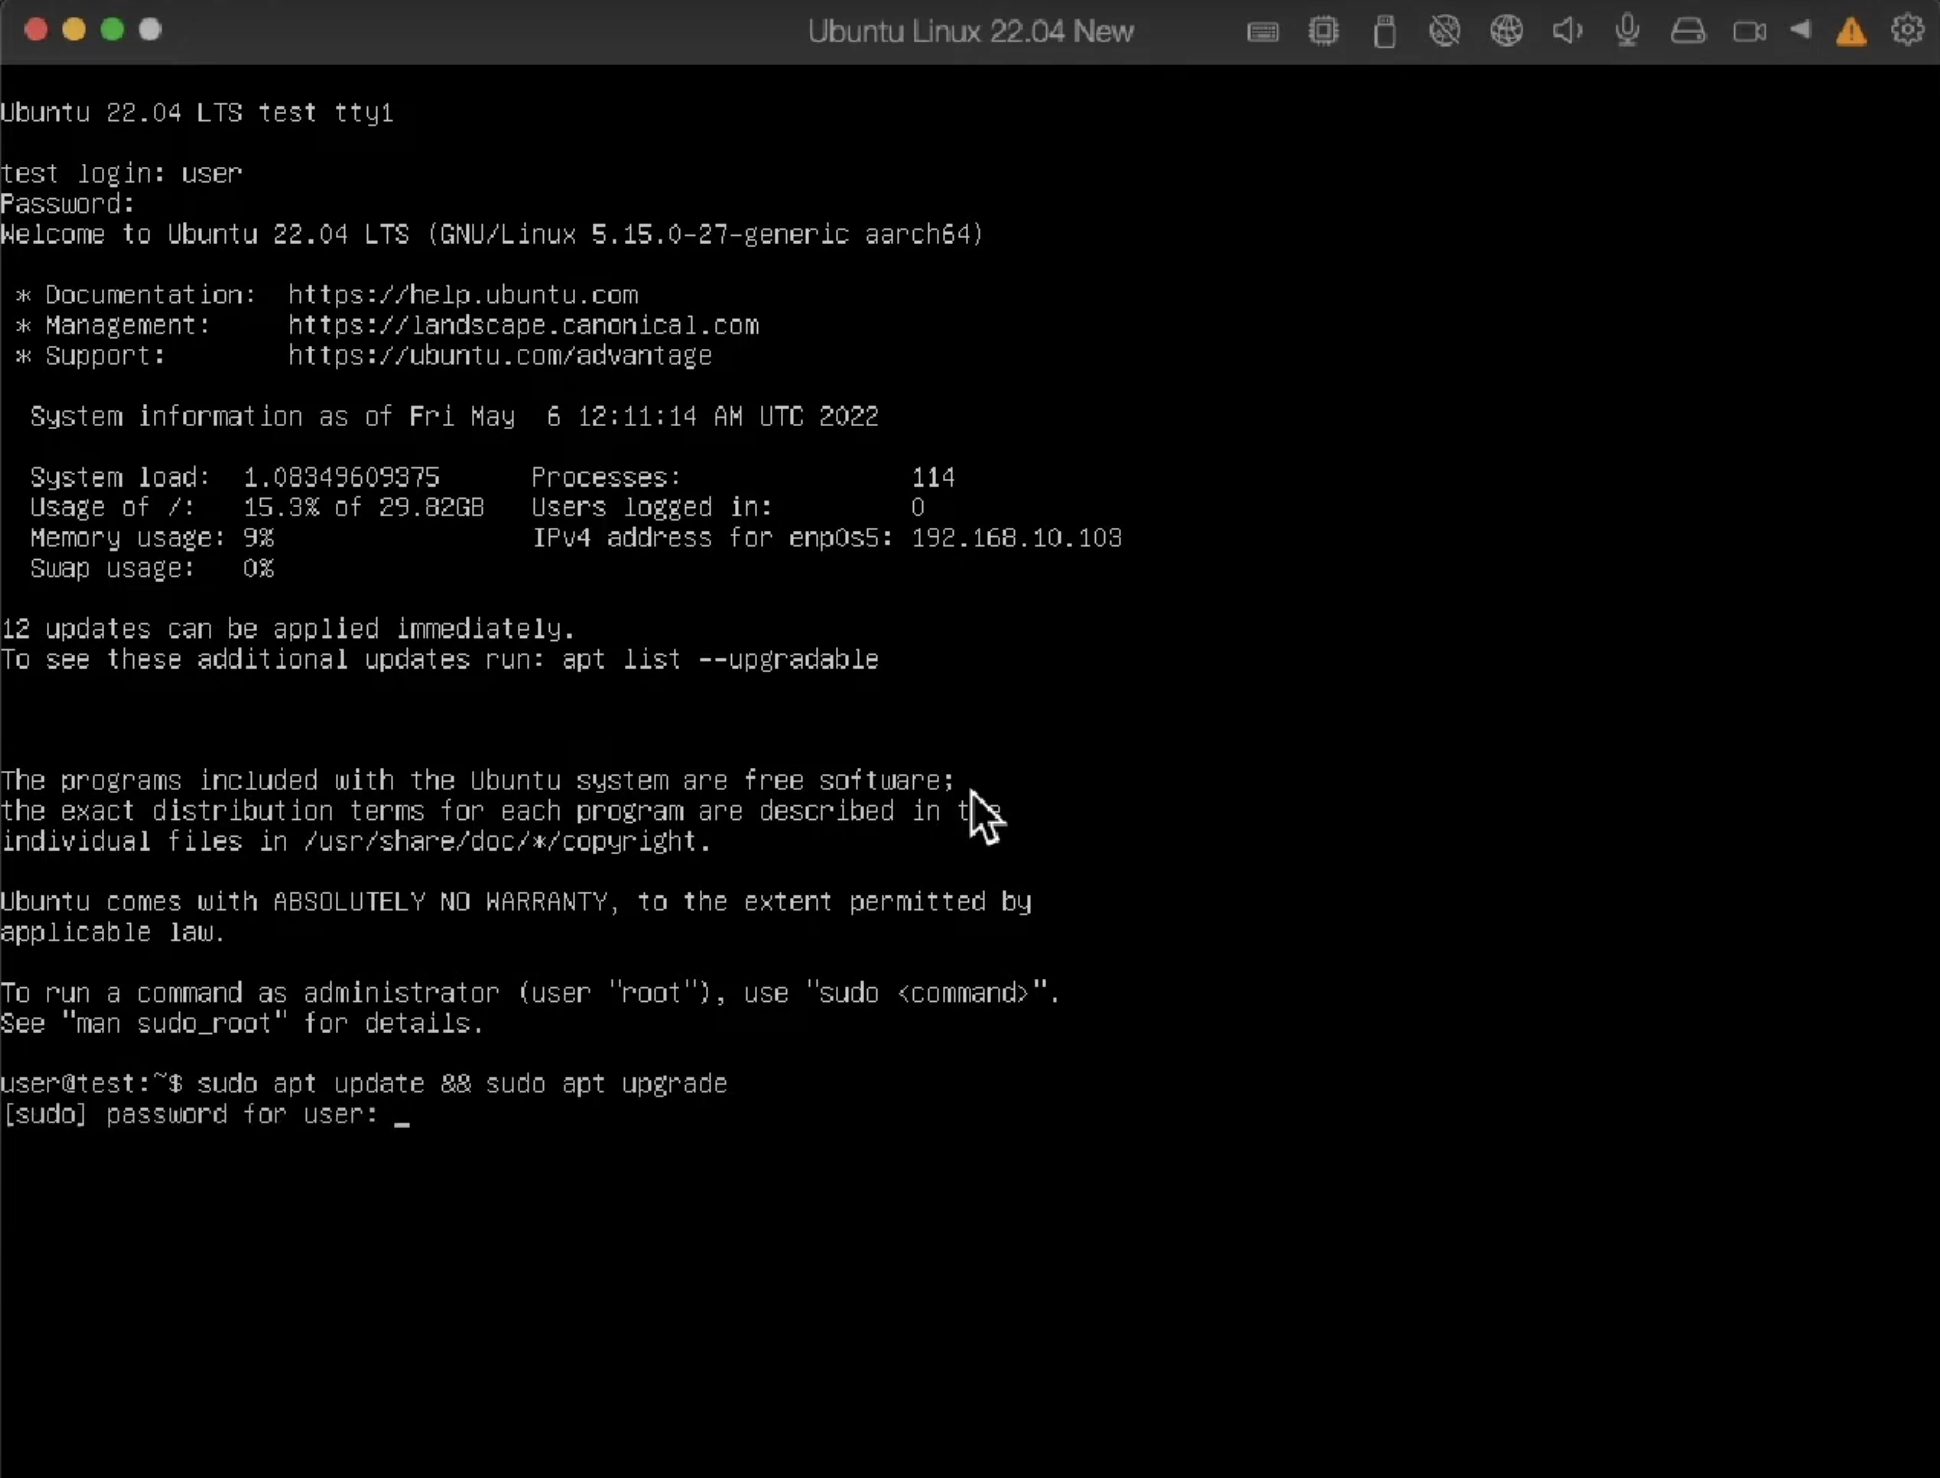
\includegraphics[width=0.5\linewidth]{images/step21.png}
        \end{figure}
    \item It will take some time to finish this step, once done, reboot using:
\begin{lstlisting}
sudo reboot
\end{lstlisting}
\end{enumerate}
\subsection{Installing the desktop image}
\begin{enumerate}
    \item You will be prompted again for the username and password to log in
    \item Install the desktop image using:
\begin{lstlisting}
sudo apt install ubuntu-desktop
\end{lstlisting}
    \begin{figure}[htp]
            \centering
            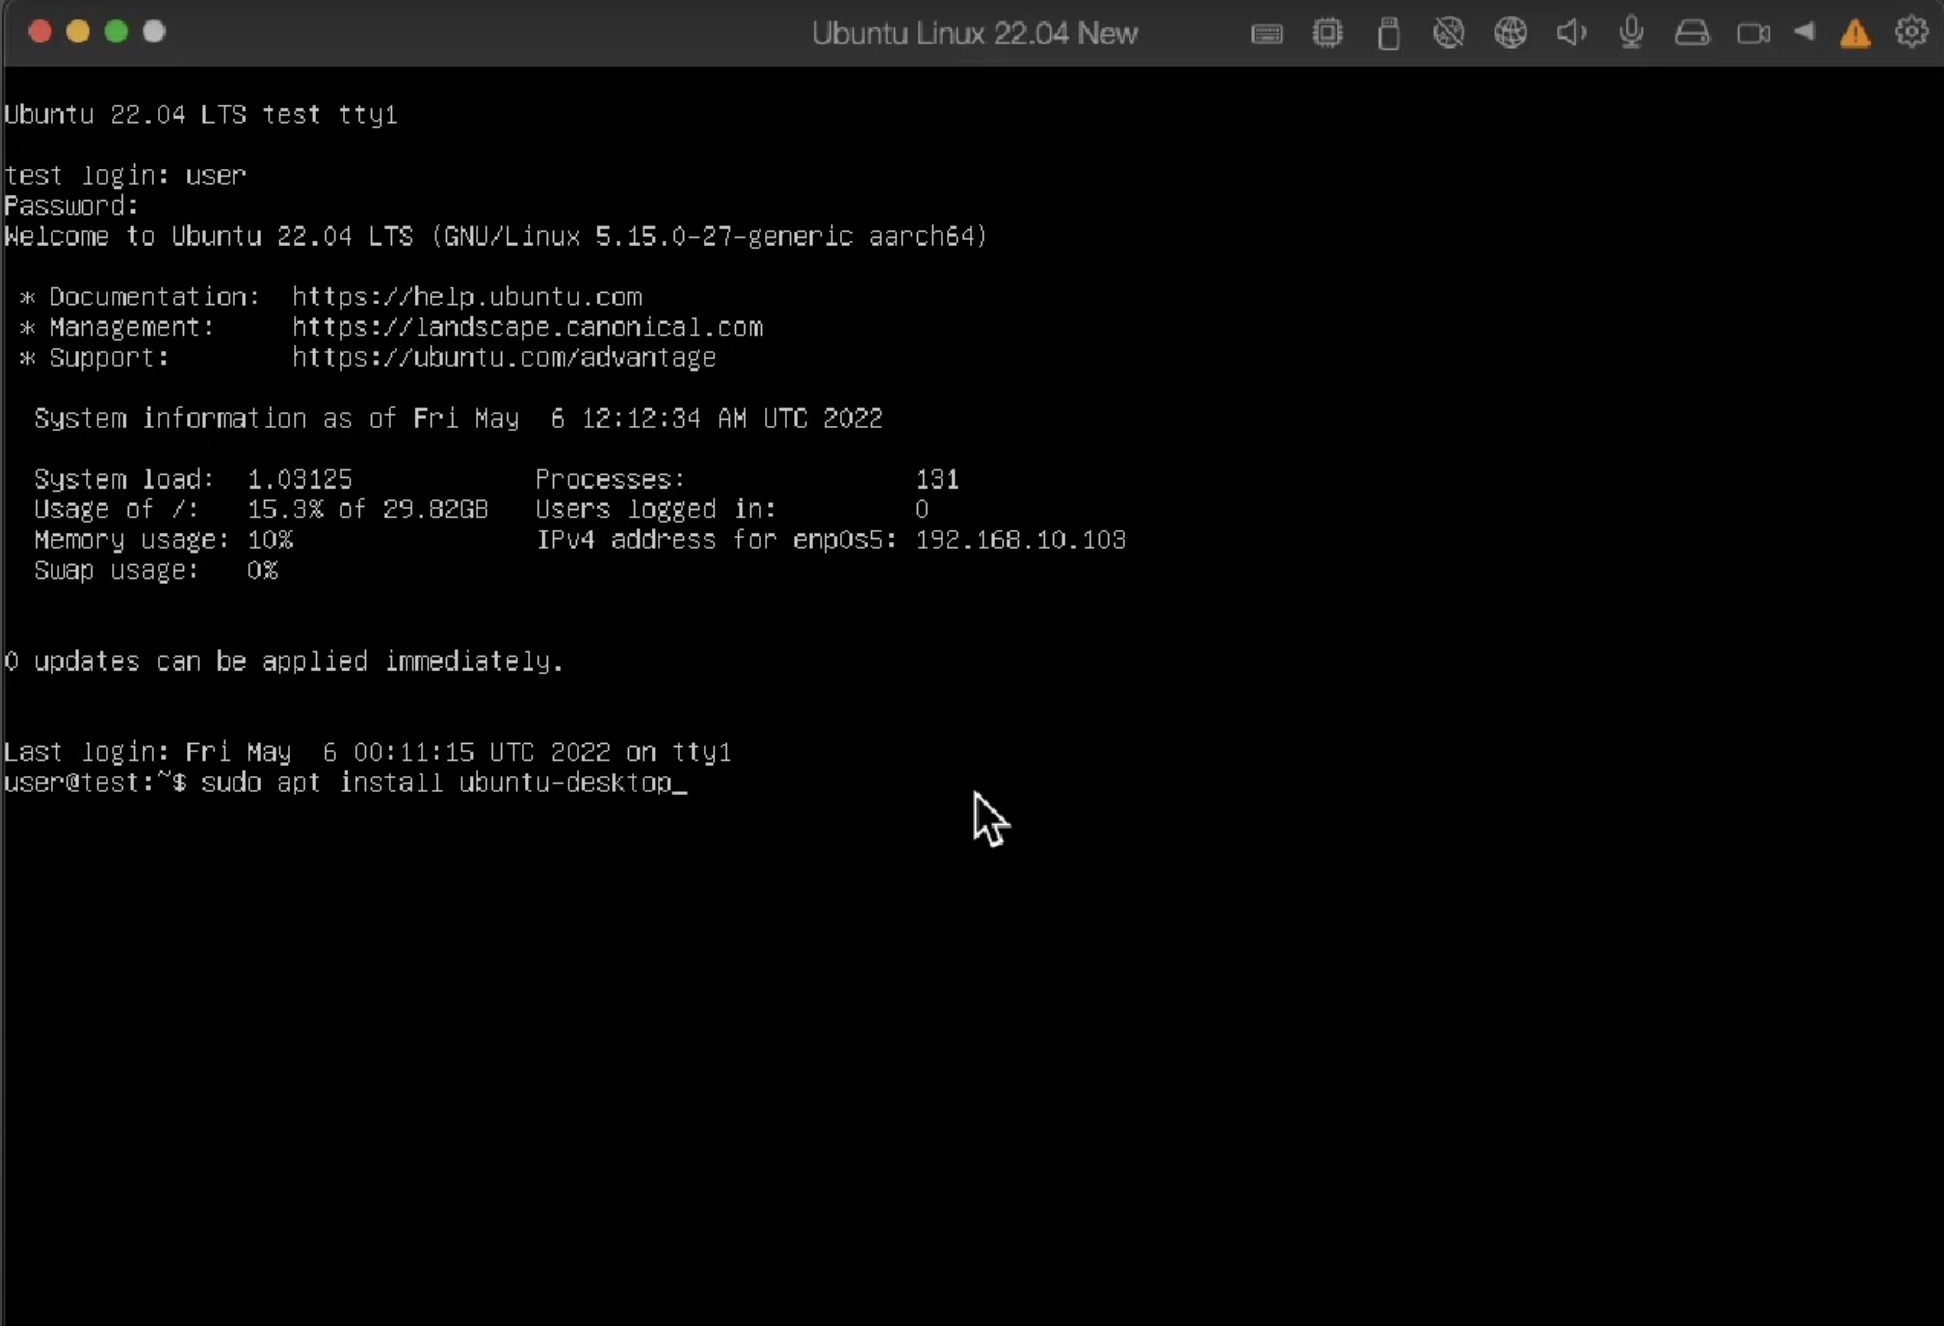
\includegraphics[width=0.6\linewidth]{images/step22.png}
        \end{figure}
    \item It will take roughly 10-15 minutes (or more depending on your internet connectivity) to finish this step, once done reboot using:
\begin{lstlisting}
sudo reboot
\end{lstlisting}
\end{enumerate}

\section{Finishing Up}
\begin{enumerate}
    \item Log in to Ubuntu:
    \begin{figure}[htp]
            \centering
            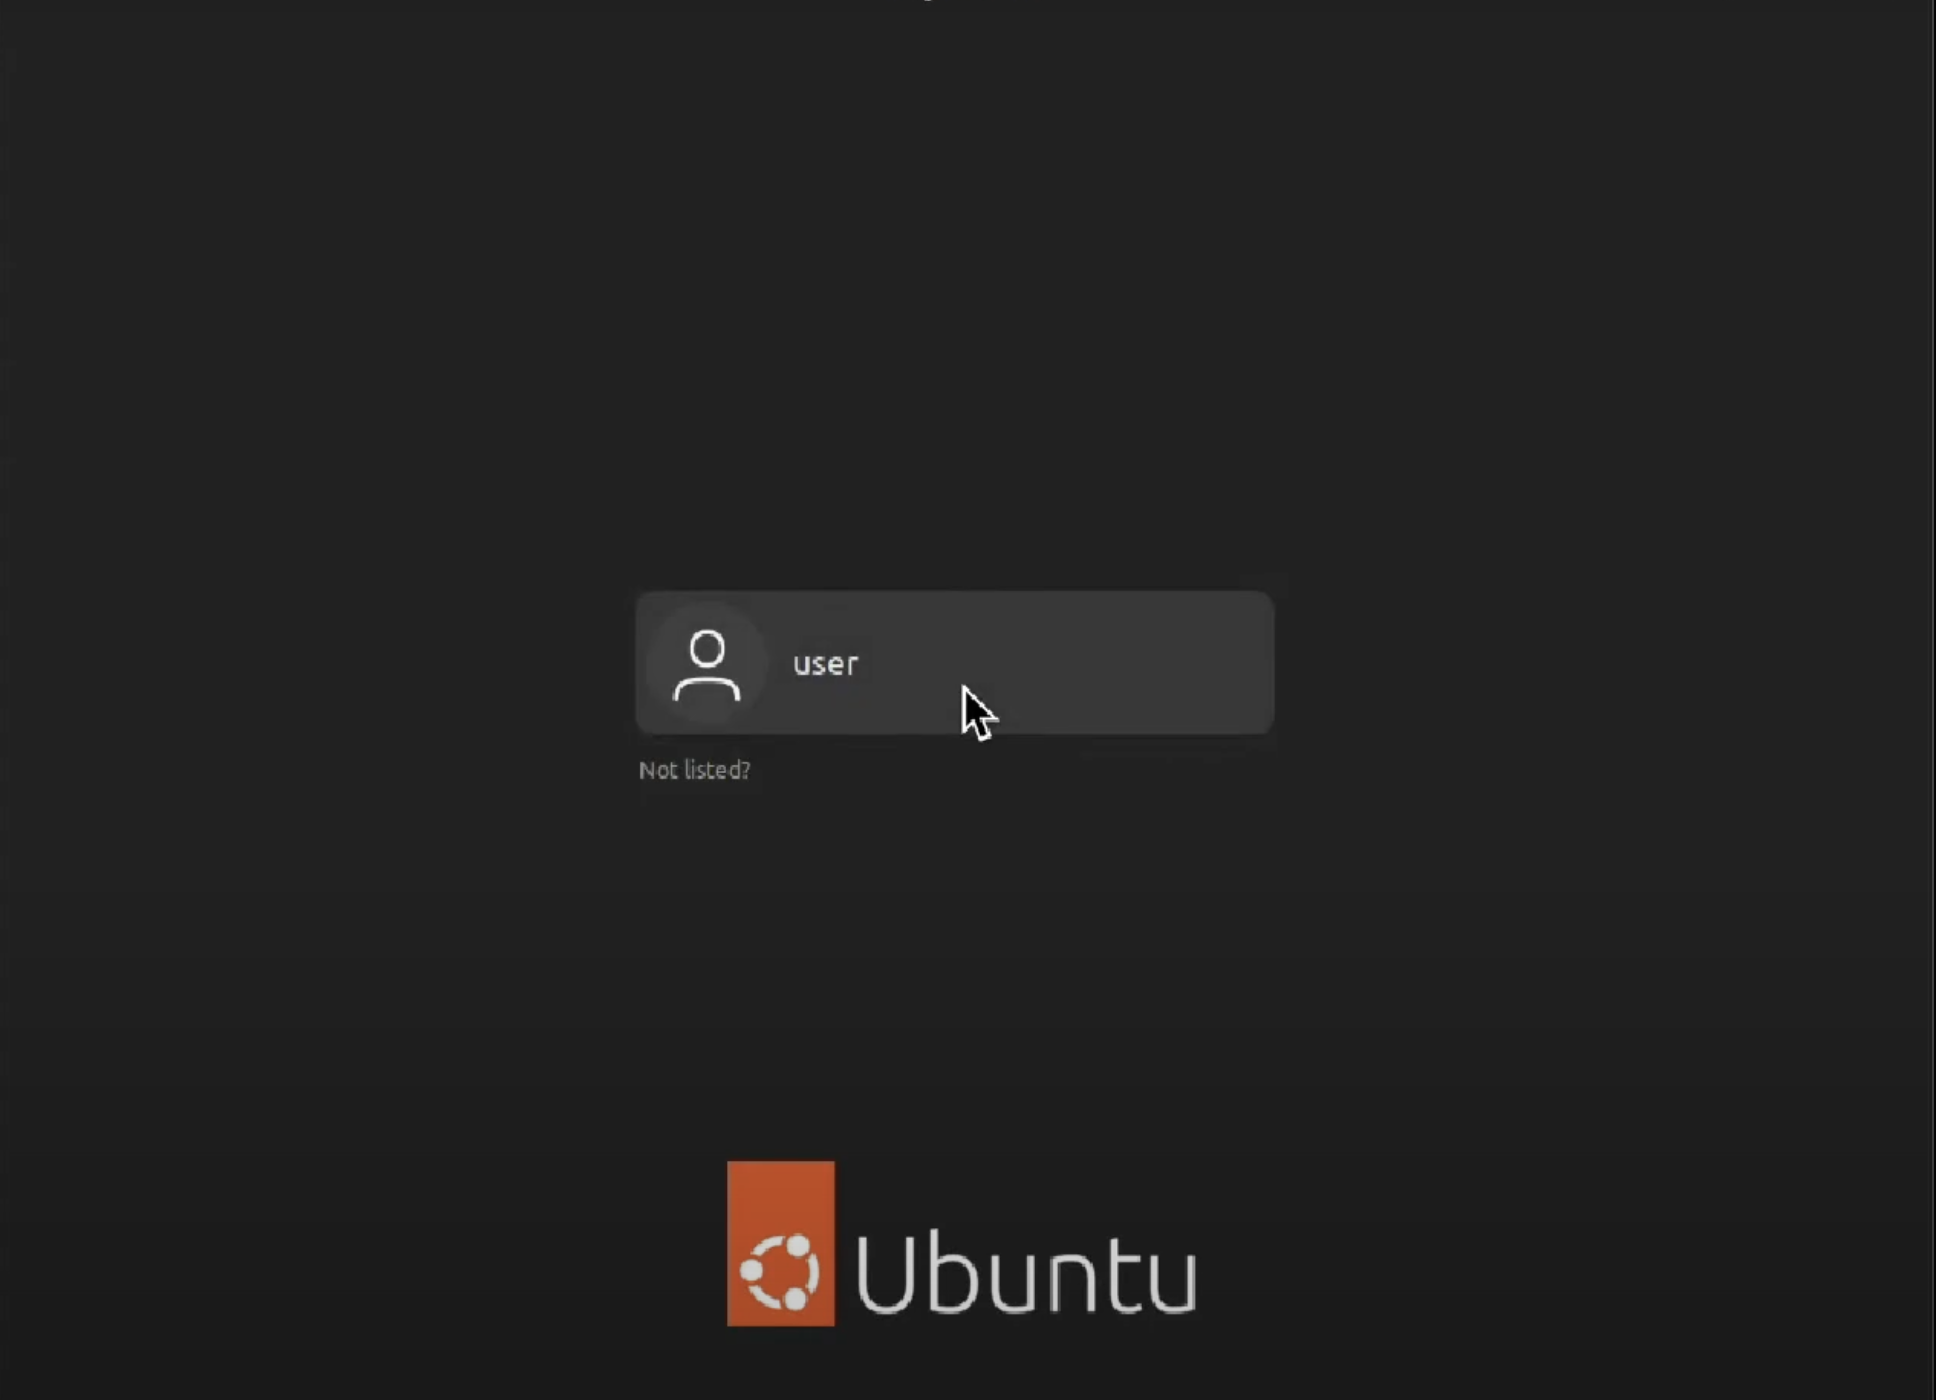
\includegraphics[width=0.6\linewidth]{images/step23.png}
        \end{figure}
    Enter the password you created earlier to log in.
    \item Follow the on-screen prompts to finalize the setup
    \begin{figure}[htp]
            \centering
            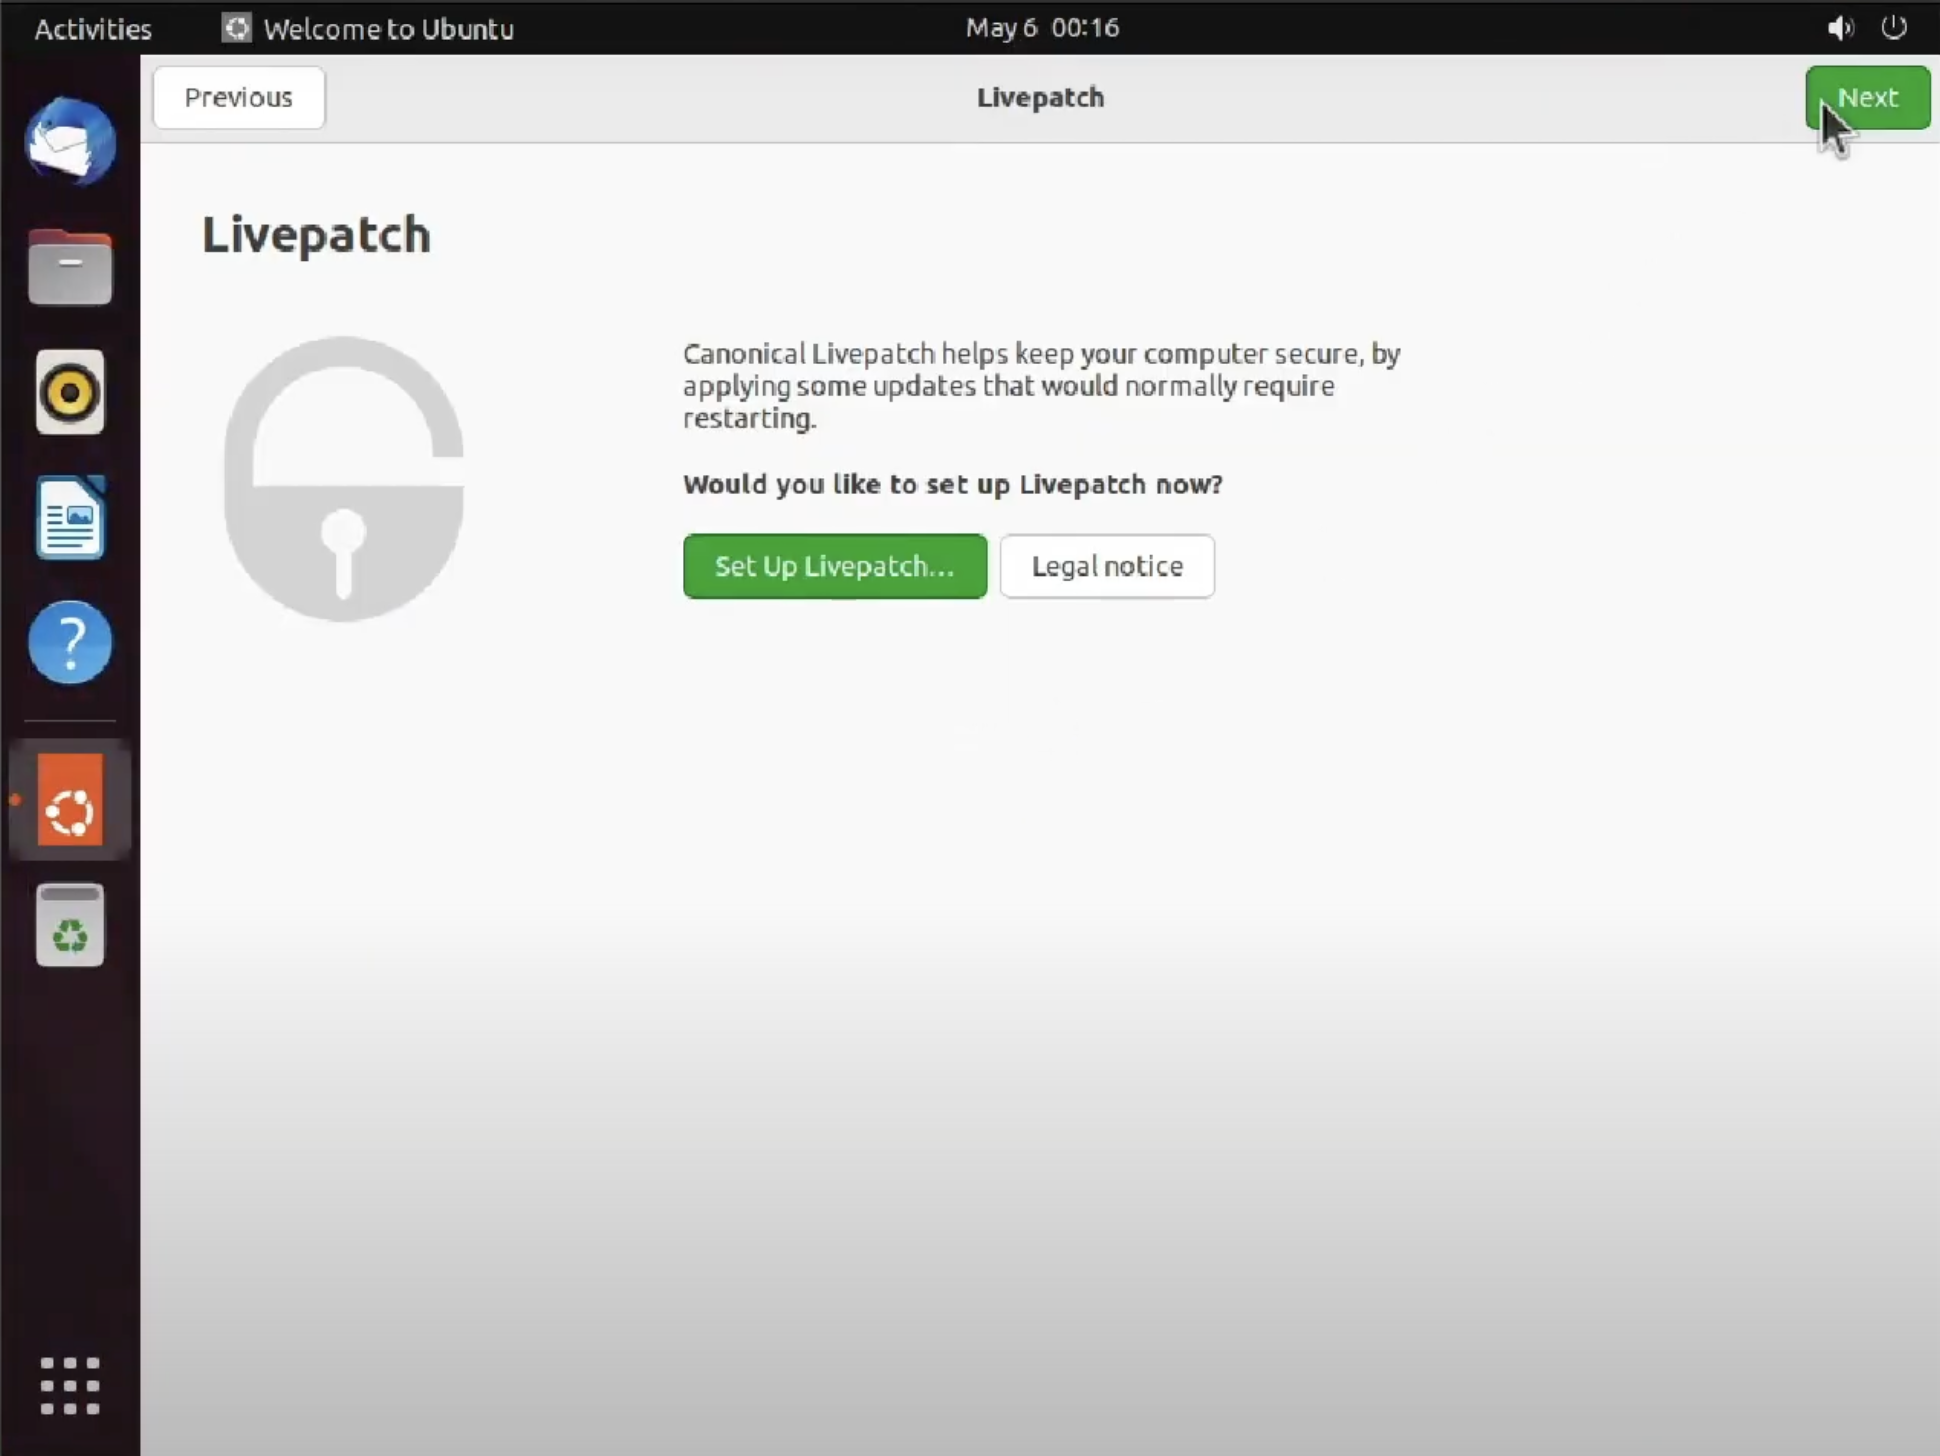
\includegraphics[width=0.6\linewidth]{images/step24.png}
        \end{figure}
    \item Reboot one final time to ensure everything is working correctly:
\begin{lstlisting}
sudo reboot
\end{lstlisting}
\end{enumerate}

\section{Troubleshooting Parallels Installation}
First contact TAs if there is any issue!
\subsection{Common Issues}
\begin{enumerate}
    \item Performance Problems:
    \begin{itemize}
        \item Check resource allocation
        \item Verify Parallels Tools installation
        \item Monitor system resources
    \end{itemize}
    \item Network Issues:
    \begin{itemize}
        \item Check network adapter settings
        \item Verify shared networking configuration
        \item Reset network settings if needed
    \end{itemize}
    \item Display Problems:
    \begin{itemize}
        \item Reinstall Parallels Tools
        \item Update graphics drivers
        \item Check resolution settings
    \end{itemize}
\end{enumerate}


\section{Advanced Parallels Features (Optional | Not Required)}
\subsection{Coherence Mode}
Coherence mode allows Ubuntu applications to run alongside macOS applications:
\begin{itemize}
    \item Enable: \textbf{View $\rightarrow$ Enter Coherence}
    \item Configure auto-start applications
    \item Set up shared applications
\end{itemize}

\subsection{Resource Management}
\begin{itemize}
    \item Adjust CPU allocation
    \item Modify RAM assignment
    \item Configure video memory
    \item Set up adaptive hypervisor
\end{itemize}

\subsection{Optimization Steps}
\begin{enumerate}
    \item Configure Display:
    \begin{itemize}
        \item Adjust resolution in Ubuntu Settings
        \item Configure scaling if needed
    \end{itemize}
    \item Enable Integration Features:
    \begin{itemize}
        \item Clipboard sharing
        \item Drag and drop support
        \item Shared folders
    \end{itemize}
\end{enumerate}

\noindent\rule{\textwidth}{1pt}

\section{ROS Installation}
Install ROS2 Jazzy Jalisco from: \hyperlink{ROS2}{https://docs.ros.org/en/jazzy/index.html}

% \section{Best Practices for Parallels Usage}
% \subsection{Performance Optimization}
% \begin{itemize}
%     \item Regular maintenance of virtual disk
%     \item Periodic cleanup of unused snapshots
%     \item Optimal resource allocation
%     \item Regular updates of both OS and Parallels
% \end{itemize}

% \subsection{Data Management}
% \begin{itemize}
%     \item Configure automated backups
%     \item Use shared folders efficiently
%     \item Implement proper snapshot strategy
% \end{itemize}
% \section{Conclusion}
% This guide covers two primary methods for running Ubuntu Linux:
% \begin{itemize}
%     \item Windows users can implement a dual-boot system
%     \item Mac users can utilize Parallels Desktop virtualization
% \end{itemize}

% Choose the method that best suits your needs and follow the appropriate sections of this guide for a successful installation.

\end{document}